% Enable tagged PDF 2.0 output. Add a formal PDF/UA standard declaration only after validation.
\DocumentMetadata{
  lang = en-US,
  pdfversion = 2.0,
  testphase = {phase-III,title,table,math,firstaid}
}
\documentclass[10pt,letterpaper]{article}
\usepackage[margin=0.75in]{geometry}
\usepackage{amsmath}
\usepackage{unicode-math}
\usepackage{array}
\usepackage{booktabs}
\usepackage{enumitem}
\usepackage{fancyhdr}
\usepackage{longtable}
\usepackage{tabularx}
\usepackage{xcolor}
\usepackage{xurl}
\usepackage{hyperref}
\usepackage{graphicx}
\usepackage[l3]{csvsimple}

\setlength{\parindent}{0pt}
%\setlength{\parskip}{0.55em}
\usepackage{parskip}
\setlist[itemize]{leftmargin=*}
\setlist[enumerate]{leftmargin=*}
\hypersetup{
  colorlinks=true,
  linkcolor=blue,
  urlcolor=blue,
  citecolor=blue,
  breaklinks=true,
  pdftitle={IVIVC App User Guide},
  pdfauthor={IVIVC App},
  pdfsubject={User guide for the IVIVC App for Absorbable Polymers},
  pdfkeywords={IVIVC, absorbable polymers, model fitting, cross-validation},
  pdfdisplaydoctitle=true
}

% All guide tables use their first row as the column-header row.
\tagpdfsetup{table/header-rows={1}}

\pagestyle{fancy}
\fancyhf{}
\lhead{IVIVC App User Guide}
\rhead{\thepage}
\fancypagestyle{plain}{\fancyhf{}\renewcommand{\headrulewidth}{0pt}}

%\renewcommand{\thesection}{\arabic{section}.}
\renewcommand{\thesubsection}{\arabic{section}.\arabic{subsection}}

\title{IVIVC App User Guide}
\author{}
\date{}

\begin{document}

\maketitle
\tableofcontents
%\newpage

% Generated by utilities/generate_user_guide.py. Edit routine wording in utilities/descriptions.yaml where possible. This is a content-only LaTeX file; include it from a top-level document. Long-form appendices are sourced from docs/appendices/; references are maintained in docs/references.bib.

\section{Introduction}

Establishing an in vitro-in vivo correlation (IVIVC) can support the evaluation of medical devices that include absorbable polymers by relating in vivo changes in material properties over time to corresponding in vitro test results, such as degradation profiles. IVIVCs may help evaluate manufacturing or material changes, support predictions of in vivo performance when modifying an existing device design, and reduce reliance on animal studies during preclinical development. This tool is intended to facilitate IVIVC development. The user supplies paired in vitro and in vivo fitting data, and may optionally supply an in vitro prediction dataset. The app applies selected preprocessing steps, fits and compares multiple correlation approaches and model families, evaluates selected performance metrics and cross-validation results, generates fitting and prediction plots, and produces report-ready summaries that can be reviewed and incorporated into external documentation.

For general background on credibility assessment and reporting of computational modeling studies in medical device submissions, see FDA guidance on computational modeling credibility and reporting \cite{fda_modeling_guidance,fda_reporting_guidance}.

\section{What the app does}

\begin{itemize}
\item Applies selected normalization, scaling, and interpolation options to prepare fitting and prediction data.
\item Fits user-selected IVIVC approaches and model families to paired in vitro and in vivo data.
\item Calculates selected goodness-of-fit, model-comparison, and cross-validation metrics.
\item Generates fitting, comparison, and prediction plots with uncertainty displays where supported.
\item Creates summaries for user-selected final approaches or models.
\end{itemize}

\section{Inputs}

The IVIVC app requires paired in vitro and in vivo degradation data, along with user-selected analysis settings that define how the data are processed, modeled, and summarized. At a high level, the inputs include:

\begin{itemize}
\item a spreadsheet containing in vitro and in vivo time-course degradation data for fitting correlations;
\item optionally, a spreadsheet containing in vitro data from which to generate predictions using fitted correlations;
\item selection of one or more IVIVC modeling approaches;
\item selection of candidate models to evaluate, where applicable;
\item optionally, preprocessing options, such as normalization, interpolation, or scaling choices;
\item selected performance metrics to display in the results and reports; by default, the app selects \(R^2\), RMSE, and AIC\textsubscript{c} as a simple starting set that has been useful in internal testing with real datasets but may not be optimal for every analysis
\item optionally, cross-validation settings for applicable parametric models; and
\item grid-search settings for model initialization.
\end{itemize}

The sections below provide additional detail on input file structure, required data columns, preprocessing options, model-selection inputs, and optional analysis settings.

\section{Outputs}

The IVIVC app generates interactive results and downloadable reports that summarize fitted model behavior, model-comparison metrics, diagnostic information, and user-selected analysis settings. Output availability depends on the selected approaches, whether fitting succeeds, and whether a prediction dataset was supplied.

\begin{longtable}{@{}>{\raggedright\arraybackslash}p{0.24\textwidth}>{\raggedright\arraybackslash}p{0.68\textwidth}@{}}
\toprule
\textbf{Output} & \textbf{Description} \\
\midrule
\endfirsthead
\toprule
\textbf{Output} & \textbf{Description} \\
\midrule
\endhead
Preprocessing outputs & Processed data tables and plots showing the data used for fitting and prediction. \\
Model fitting outputs & Parameter estimates, parameter standard errors where available, fitted plots, residual (error) plots, and selected performance metrics. \\
Model comparison outputs & Tables comparing selected approaches, models, metrics, and cross-validation summaries. \\
Prediction outputs & Prediction plots and downloadable tables when a prediction dataset is supplied and the selected method can be applied. \\
Selected model \& summary of outputs & User-selected report summaries and optional Word report export for incorporation into external documentation. \\
\bottomrule
\end{longtable}

\section{Input datasets}

\begin{longtable}{@{}>{\raggedright\arraybackslash}p{0.24\textwidth}>{\raggedright\arraybackslash}p{0.68\textwidth}@{}}
\toprule
\textbf{Input} & \textbf{Description} \\
\midrule
\endfirsthead
\toprule
\textbf{Input} & \textbf{Description} \\
\midrule
\endhead
Fitting dataset & Required four-column dataset used to establish the in vitro/in vivo relationship. Columns are interpreted as in vitro time, in vitro value, in vivo time, and in vivo value. \\
Prediction dataset & Optional two-column in vitro dataset used after fitting to generate in vivo predictions. Columns are interpreted as in vitro time and in vitro value. \\
\bottomrule
\end{longtable}

For Excel workbooks, select the sheet containing the relevant data. For CSV files, the first columns are read directly in the order described above.

\section{Analysis approaches and models}

\begin{longtable}{@{}>{\raggedright\arraybackslash}p{0.18\textwidth}>{\raggedright\arraybackslash}p{0.46\textwidth}>{\raggedright\arraybackslash}p{0.28\textwidth}@{}}
\toprule
\textbf{Approach} & \textbf{Description} & \textbf{Available models} \\
\midrule
\endfirsthead
\toprule
\textbf{Approach} & \textbf{Description} & \textbf{Available models} \\
\midrule
\endhead
Approach 1: Direct Correlation & Approach 1 fits a direct relationship between matched in vitro and in vivo time points after preprocessing. The fitted model is then used as a time-scaling function that maps an in vitro time to a predicted in vivo time. & Double Exponential, Exponential, Linear, Linear (zero intercept), Power \\
Approach 2: Independent Model Fitting & Approach 2 fits the same model family independently to the in vitro and in vivo datasets. With fitting data alone, the report summarizes the two fitted models and their fitted-curve uncertainty. When prediction data are supplied, predictions can be generated by comparing the fitted in vivo and in vitro responses or by comparing fitted characteristic time constants when those values are available. & Double Exponential, Exponential, Mass Loss (Gompertz), Mass Loss (One-Phase), Mass Loss (Surface Erosion), Mass Loss (Two-Phase), Power, Stretched Exponential \\
Approach 3: Direct Mapping & Approach 3 uses direct interpolation-based mappings between datasets rather than fitting a parametric model. It can describe value-ratio behavior over time and time-ratio behavior over value ranges. When prediction data are supplied, those mappings can be used to scale prediction values or prediction times. & No parametric model selection \\
\bottomrule
\end{longtable}

\subsection{Candidate model functional forms}

\begin{longtable}{@{}>{\raggedright\arraybackslash}p{0.16\textwidth}>{\raggedright\arraybackslash}p{0.14\textwidth}>{\raggedright\arraybackslash}p{0.36\textwidth}>{\raggedright\arraybackslash}p{0.26\textwidth}@{}}
\toprule
\textbf{Model} & \textbf{Used in} & \textbf{Functional form} & \textbf{Notes} \\
\midrule
\endfirsthead
\toprule
\textbf{Model} & \textbf{Used in} & \textbf{Functional form} & \textbf{Notes} \\
\midrule
\endhead
Double Exponential & Approach 1, Approach 2 & \(y = a e^{b x} + c e^{d x}\) & Sum of two exponential terms. It can represent profiles with two apparent rates, but the added flexibility may require more data to estimate stably. \\
Exponential & Approach 1, Approach 2 & \(y = a e^{b x}\) & Two-parameter exponential relationship. It can describe monotonic change that accelerates or decelerates exponentially over the fitted range. \\
Linear & Approach 1 & \(y = a + b x\) & Straight-line empirical relationship with an intercept and slope. It is appropriate when the in vitro/in vivo relationship is approximately linear over the fitted range. \\
Linear (zero intercept) & Approach 1 & \(y = a x\) & Straight-line empirical relationship constrained to pass through zero. It may be useful when a zero in vitro value should correspond to a zero in vivo value under the selected preprocessing and response scale. \\
Mass Loss (Gompertz) & Approach 2 & \(y = y_0 - A \exp\{-\exp[(e r_{max}/A)(t_{lag}-x)+1]\}\) & Mass-remaining model based on the modified Gompertz curve. It is intended for asymmetric sigmoidal mass-loss profiles with an apparent lag or plateau, a maximum loss-rate region, and a terminal loss extent. \\
Mass Loss (One-Phase) & Approach 2 & \(y = y_0 - A/(1 + e^{-(x-t_{50})/s})\) & Mass-remaining model with a delayed sigmoidal loss phase. It is intended for mass-loss profiles that begin constant and show a later drop. \\
Mass Loss (Surface Erosion) & Approach 2 & \(y = y_0 \max(1-kx,0)^n\) & Mass-remaining model for surface-controlled erosion. The fitted exponent n allows the profile shape to adapt to slab-like, cylindrical, spherical, or empirical geometry-like erosion behavior. \\
Mass Loss (Two-Phase) & Approach 2 & \(y = y_0 - B(1-e^{-k_b x}) - D/(1+e^{-(x-t_{50})/s})\) & Mass-remaining model with an optional early burst-loss phase followed by a delayed sigmoidal loss phase. It is intended for mass-loss profiles that may show an initial drop, an intermediate plateau, and a later drop. \\
Power & Approach 1, Approach 2 & \(y = a x^{b}\) & Power-law empirical relationship. It can describe nonlinear monotonic relationships where the response changes as a fitted power of time or the mapped predictor. \\
Stretched Exponential & Approach 2 & \(y = a e^{b x^{c}}\) & Exponential relationship with a fitted stretching exponent. It can describe non-single-rate behavior, but the additional shape parameter can increase sensitivity when data are sparse. \\
\bottomrule
\end{longtable}

\textbf{Mass-loss model source notes}

The surface-erosion mass-loss form is based on geometry-controlled surface erosion concepts such as the erodible slab, cylinder, and sphere model \cite{hopfenberg1976}. The one-phase mass-loss model uses a logistic/sigmoidal transition to represent a delayed loss phase \cite{tsoularis2002}. The two-phase mass-loss model combines an early burst-like loss term with a delayed sigmoidal loss phase. Burst and delayed/multiphase behavior in degradable polymer systems is discussed in the polymer erosion and PLGA release literature \cite{gopferich1997,fredenberg2011,allison2008}. The Gompertz mass-loss model uses a modified Gompertz-style sigmoidal form with lag and maximum-rate parameters \cite{zwietering1990}.

\section{Preprocessing options}

\subsection{Normalization}

\begin{longtable}{@{}>{\raggedright\arraybackslash}p{0.22\textwidth}>{\raggedright\arraybackslash}p{0.20\textwidth}>{\raggedright\arraybackslash}p{0.50\textwidth}@{}}
\toprule
\textbf{Option} & \textbf{Internal key} & \textbf{Description} \\
\midrule
\endfirsthead
\toprule
\textbf{Option} & \textbf{Internal key} & \textbf{Description} \\
\midrule
\endhead
Min-max normalization & min\_max & Scales response values to the 0-1 range using the observed minimum and maximum within each dataset. \\
Initial-value normalization & initial\_value & Divides response values by the first response value in the corresponding dataset. \\
\bottomrule
\end{longtable}

\subsection{Scaling}

\begin{longtable}{@{}>{\raggedright\arraybackslash}p{0.22\textwidth}>{\raggedright\arraybackslash}p{0.20\textwidth}>{\raggedright\arraybackslash}p{0.50\textwidth}@{}}
\toprule
\textbf{Option} & \textbf{Internal key} & \textbf{Description} \\
\midrule
\endfirsthead
\toprule
\textbf{Option} & \textbf{Internal key} & \textbf{Description} \\
\midrule
\endhead
Log10 time scaling & log\_x & Applies a base-10 logarithm to time values before fitting or interpolation. \\
Log10 response scaling & log\_y & Applies a base-10 logarithm to response values before fitting or interpolation. \\
\bottomrule
\end{longtable}

\subsection{Interpolation}

\begin{longtable}{@{}>{\raggedright\arraybackslash}p{0.22\textwidth}>{\raggedright\arraybackslash}p{0.20\textwidth}>{\raggedright\arraybackslash}p{0.50\textwidth}@{}}
\toprule
\textbf{Option} & \textbf{Internal key} & \textbf{Description} \\
\midrule
\endfirsthead
\toprule
\textbf{Option} & \textbf{Internal key} & \textbf{Description} \\
\midrule
\endhead
No interpolation & none & Uses only exact raw alignments. No values are estimated between observations; unavailable aligned positions are marked as missing. \\
Shared-time interpolation & default & Interpolates both datasets onto the common set of experimental time points, using linear interpolation and marking out-of-range values as unavailable. \\
Densified interpolation & alternative & Creates additional linearly spaced points between adjacent observations before interpolation. This can smooth displays and make fitting more stable, but adds more interpolation-derived points that skew statistical comparisons. \\
\bottomrule
\end{longtable}

\section{Relative model evidence}

Relative model evidence compares candidate parametric models fitted to the same dataset under the same preprocessing settings and IVIVC approach. The evidence table is based only on the information-criterion metrics selected by the user: AIC, AIC\textsubscript{c}, and/or BIC. These criteria are relative; their absolute values are not interpreted directly, and negative values are allowed. Table definitions: n is the number of fitted observations; k is the number of fitted model parameters; Delta is the difference between a model's criterion value and the lowest value in the displayed candidate set; weight is the normalized relative support for that model under the criterion; and evidence ratio compares the highest weight in the set with the model's weight. Delta values near 0 indicate similar relative support; larger delta values indicate lower support relative to the leading candidate under that criterion. Similar relative evidence does not mean the models are scientifically equivalent. Final model selection should also consider prediction error, cross-validation behavior, residual patterns, parameter uncertainty, model simplicity, and biological or degradation-mechanism plausibility. The app reports these summaries to support user review. It does not select, recommend, or validate a model.

For additional background on information criteria, model-selection evidence, and evidence-weight interpretation, see references \cite{akaike1974,schwarz1978,burnham2002,kass1995,wagenmakers2004}.

\begin{longtable}{@{}>{\raggedright\arraybackslash}p{0.24\textwidth}>{\raggedright\arraybackslash}p{0.68\textwidth}@{}}
\toprule
\textbf{Evidence summary} & \textbf{Interpretation} \\
\midrule
\endfirsthead
\toprule
\textbf{Evidence summary} & \textbf{Interpretation} \\
\midrule
\endhead
Delta AIC\textsubscript{c} / Delta AIC / Delta BIC & Difference from the lowest value in the displayed candidate set. Values near 0 indicate similar relative support; larger values indicate lower support relative to the leading candidate under that criterion. \\
AIC\textsubscript{c} or BIC weight & Normalized relative-support value across the candidate models in the displayed evidence table. Weights are relative, not absolute probabilities that a model is true. \\
Evidence ratio & Ratio of the highest evidence weight to the model's evidence weight. Larger ratios indicate less relative support compared with the highest-weighted model in the set. \\
Interpretation badge & Neutral rule-of-thumb label based on the displayed delta values. The label supports user review and is not an app recommendation. \\
\bottomrule
\end{longtable}

\section{Cross-validation options}

Cross-validation provides an approximate check of how a fitted model performs on held-out data. It is most useful when there are enough observations to fit the model repeatedly while leaving some observations out for evaluation.

The available schemes are Leave-one-timepoint-out, Leave-contiguous-block-out, Shuffle split, K-fold, and None. Leave-one-timepoint-out holds out one observation at a time, Leave-contiguous-block-out holds out adjacent time points, Shuffle split uses repeated random holdout sets, K-fold uses ordered fold-based holdouts, and None disables cross-validation. The block-size setting for Leave-contiguous-block-out controls how many consecutive observations are held out in each split. Larger blocks may leave too few observations for stable fitting, especially in small datasets. For small datasets, cross-validation summaries should be interpreted as exploratory diagnostics rather than definitive validation results.

Leave-one-timepoint-out is the default cross-validation scheme. It is a practical starting point for small time-course datasets because each split uses all but one observation for fitting. Leave-contiguous-block-out and K-fold can be used as more demanding time-region holdout checks, while Shuffle split is retained as a familiar exploratory option.

For background on cross-validation procedures and their use in model assessment and selection, particularly for for time series, see references \cite{arlot2010, bergmeir2012, roberts2017, bergmeir2018}.

\begin{longtable}{@{}>{\raggedright\arraybackslash}p{0.20\textwidth}>{\raggedright\arraybackslash}p{0.20\textwidth}>{\raggedright\arraybackslash}p{0.52\textwidth}@{}}
\toprule
\textbf{Scheme} & \textbf{Internal key} & \textbf{Description} \\
\midrule
\endfirsthead
\toprule
\textbf{Scheme} & \textbf{Internal key} & \textbf{Description} \\
\midrule
\endhead
Leave-one-timepoint-out & leave\_one\_timepoint\_out & Holds out one time point at a time and fits the model using all remaining time points. This is the default because it uses as much data as possible for fitting while still providing a held-out prediction diagnostic for small time-course datasets. \\
Leave-contiguous-block-out & leave\_contiguous\_block\_out & Holds out adjacent time points as a block in x-axis order. The block-size setting controls how many adjacent observations are held out in each split. The maximum useful block size depends on the number of observations. Larger blocks may leave too few observations for stable fitting, especially in small datasets. \\
Shuffle split & shuffle\_split & Repeatedly creates random training and holdout subsets. This can be useful as an exploratory sensitivity check when the dataset has enough observations to support repeated resampling. The splits, test-size, and random-seed settings control the repeated random holdouts. \\
K-fold & kfold & Divides the ordered dataset into a specified number of folds, fits the model on all but one fold, and evaluates on the held-out fold. With small k, this can act as a more demanding time-region holdout test. \\
None & none & Disables cross-validation. This may be appropriate when the dataset is too small for meaningful holdout validation or when only fitted-model summaries are needed. \\
\bottomrule
\end{longtable}

\begin{longtable}{@{}>{\raggedright\arraybackslash}p{0.22\textwidth}>{\raggedright\arraybackslash}p{0.22\textwidth}>{\raggedright\arraybackslash}p{0.48\textwidth}@{}}
\toprule
\textbf{Parameter} & \textbf{Internal key} & \textbf{Description} \\
\midrule
\endfirsthead
\toprule
\textbf{Parameter} & \textbf{Internal key} & \textbf{Description} \\
\midrule
\endhead
Cross-validation scheme & cv\_scheme & Selects the splitting method used to estimate held-out performance for fitted parametric models. Leave-one-timepoint-out is the default. \\
CV splits/folds/block size & cv\_n\_splits & For Shuffle split, the number of repeated random train/test splits. For K-fold, the number of folds. For Leave-contiguous-block-out, the number of adjacent time points held out per split. The setup page does not enforce a maximum block size because the uploaded data are not read until Analyze is selected; larger blocks may leave too few observations for stable fitting. This setting is not used for Leave-one-timepoint-out or None. \\
Shuffle split test size & cv\_test\_size & The fraction of observations held out for testing in each Shuffle split repeat. Smaller values leave more observations for fitting; larger values make the holdout test more demanding but leave fewer observations for training. \\
CV random seed & cv\_random\_state & Seed used to make randomized cross-validation splits reproducible. This applies to Shuffle split. \\
\bottomrule
\end{longtable}

\section{Grid-search initialization}

The app conducts an automated grid search to identify suitable starting parameter values for each model before nonlinear least-squares fitting, reducing the need for manual parameter tuning. Candidate values are sampled within the configured parameter bounds and are used only to initialize the final curve fit.

This initialization step improves convergence and reduces sensitivity to poor starting values. It is not itself the final fitting algorithm and does not guarantee that the final fitted parameters are the global optimum.

\begin{longtable}{@{}>{\raggedright\arraybackslash}p{0.24\textwidth}>{\raggedright\arraybackslash}p{0.24\textwidth}>{\raggedright\arraybackslash}p{0.44\textwidth}@{}}
\toprule
\textbf{Parameter} & \textbf{Internal key} & \textbf{Description} \\
\midrule
\endfirsthead
\toprule
\textbf{Parameter} & \textbf{Internal key} & \textbf{Description} \\
\midrule
\endhead
Grid-search random starts & grid\_search\_num\_points & Number of candidate starting parameter sets evaluated before nonlinear least-squares fitting. Higher values may improve robustness but increase runtime. \\
Grid-search CPU cores & grid\_search\_num\_cores & Number of CPU cores used for the starting-point search. Blank or Auto uses the app default. \\
Grid-search parameter minimum & grid\_search\_param\_min & Lower bound for randomly sampled candidate starting parameter values. \\
Grid-search parameter maximum & grid\_search\_param\_max & Upper bound for randomly sampled candidate starting parameter values. \\
Grid-search random seed & grid\_search\_random\_state & Seed used to make randomized starting-point sampling reproducible. Changing the seed changes the sampled candidates while keeping the same bounds and number of starts. \\
\bottomrule
\end{longtable}

\section{Performance metrics}

By default, the app selects \(R^2\), RMSE, and AIC\textsubscript{c}. This compact default set has been simple and useful in internal testing with real datasets, but it is not necessarily the best set for every dataset or intended use. Users may select additional metrics when they provide useful context for a specific analysis.

\begin{longtable}{@{}>{\raggedright\arraybackslash}p{0.17\textwidth}>{\raggedright\arraybackslash}p{0.18\textwidth}>{\raggedright\arraybackslash}p{0.20\textwidth}>{\raggedright\arraybackslash}p{0.37\textwidth}@{}}
\toprule
\textbf{Metric} & \textbf{Internal key} & \textbf{Preferred direction} & \textbf{Description} \\
\midrule
\endfirsthead
\toprule
\textbf{Metric} & \textbf{Internal key} & \textbf{Preferred direction} & \textbf{Description} \\
\midrule
\endhead
\(R^2\) & r\_squared & Higher is better & Coefficient of determination. Higher values indicate that the model explains more variance in the observed response. \\
Adjusted \(R^2\) & adjusted\_r\_squared & Higher is better & \(R^2\) adjusted for the number of fitted parameters, which can penalize unnecessary model complexity. \\
MSE & mse & Lower is better & Mean squared error between observed and fitted values. Lower values indicate smaller average squared residuals. \\
RMSE & rmse & Lower is better & Root mean squared error, in the same response units as the fitted data. Lower values indicate smaller typical residuals. \\
MAE & mae & Lower is better & Mean absolute error, in the same response units as the fitted data. Lower values indicate smaller average absolute residuals. \\
NRMSE (mean) & mnrmse & Lower is better & RMSE normalized by the response mean. Lower values indicate smaller error relative to the response magnitude. \\
NRMSE (std. dev.) & nrmse & Lower is better & RMSE normalized by the response standard deviation. Lower values indicate smaller error relative to response variability. \\
AIC & aic & Lower is better & Akaike Information Criterion. Information-criterion metrics balance how well a model fits the data with model complexity (the number of fitted parameters). Among comparable fitted models, a lower AIC value generally indicates a better model representation: the model explains the data well without unnecessary complexity. Absolute AIC values, including negative values, should not be interpreted as standalone quality grades. \\
AIC\textsubscript{c} & aicc & Lower is better & Corrected Akaike Information Criterion. AIC\textsubscript{c} applies a small-sample correction to AIC and is often preferred when the number of fitted observations (n) is limited relative to the number of fitted parameters (k), with n/k < 40 commonly used as a rule of thumb. Among comparable fitted models, a lower AIC\textsubscript{c} value generally indicates a better balance of fit quality and model complexity; AIC\textsubscript{c} is undefined when there are too few observations relative to the number of parameters. \\
BIC & bic & Lower is better & Bayesian Information Criterion. BIC balances how well a model fits the data with model complexity, usually applying a stronger penalty for additional parameters than AIC. Among comparable fitted models, a lower BIC value generally indicates a better model representation without unnecessary complexity. Absolute BIC values, including negative values, should not be interpreted as standalone quality grades. \\
\bottomrule
\end{longtable}

For additional background on common error metrics, scale-dependent accuracy measures, and adjusted \(R^2\), see references \cite{hodson2022,hyndman2006,miles2014}.

For AIC\textsubscript{c}, a commonly cited rule of thumb is to prefer AIC\textsubscript{c} over AIC when the ratio of fitted observations to estimated parameters is small, such as \(n/k < 40\), where \(n\) is the number of fitted observations and \(k\) is the number of estimated model parameters \cite{burnham2002}.

\section{Uncertainty and error bars}

The following descriptions summarize how fitted-parameter uncertainty, fitting-plot bands, and prediction error bars are calculated or interpreted for each approach.

\subsection{Approach 1: Direct Correlation}

\textbf{Fitting uncertainty}

Parameter estimates: fitted parameters are reported as estimate \(\pm\) standard error. Standard errors are derived from the nonlinear least-squares parameter covariance matrix. Correlations among fitted parameters are retained when uncertainty-aware parameter values are created.

Fitting plot bands: shaded 95\% prediction bands are generated by Monte Carlo sampling of the fitted parameter covariance matrix. The sampled model variance is combined with the residual variance from the fitted data, then converted to a two-sided interval using a t multiplier when residual degrees of freedom are available.

These bands describe approximate prediction uncertainty around the fitted relationship, not regulatory acceptance limits. They depend on the fitted model form, local covariance approximation, residual behavior, and preprocessing choices.

\textbf{Prediction uncertainty}

Prediction plot error bars: when a prediction dataset is supplied, predicted in vivo times are plotted with horizontal error bars. The bars are calculated from the same 95\% prediction-band calculation used for the fitted correlation model; the upper and lower bar lengths are the distances from the band mean to the corresponding upper and lower interval bounds at each input prediction time.

The error bars therefore include propagated fitted-parameter uncertainty and residual/model error from the Approach 1 correlation fit.

\subsection{Approach 2: Independent Model Fitting}

\textbf{Fitting uncertainty}

Parameter estimates: each in vitro and in vivo model parameter is reported as estimate \(\pm\) standard error. Standard errors are derived from the corresponding nonlinear least-squares covariance matrix, with fitted-parameter correlations retained in uncertainty-aware values.

Time constants: tau values, when available, are calculated from the fitted model and parameter covariance. The reported tau uncertainty is the propagated standard uncertainty from that covariance-based calculation.

Fitting plot bands: the in vitro and in vivo shaded 95\% prediction bands are generated separately. For each fitted model, the app Monte Carlo samples the fitted parameter covariance matrix, combines sampled model variance with residual variance, and converts the resulting standard uncertainty to a two-sided interval using a t multiplier when residual degrees of freedom are available.

\textbf{Prediction uncertainty}

Value-ratio prediction error bars: uncertainty is propagated from both fitted models. The app samples each model's parameter covariance matrix, calculates the in vivo/in vitro response ratio for each sample, combines ratio variance with residual-based ratio uncertainty, and converts that uncertainty to a two-sided 95\% interval. The plotted vertical error bars are scaled from the resulting ratio interval at each prediction time.

Time-constant-ratio prediction error bars: when both tau values are valid, uncertainty in each tau is propagated through the tau ratio using uncertainty-aware arithmetic. The standard uncertainty of the scaled prediction time is multiplied by a t value, where available, and plotted as a symmetric horizontal error bar.

Ratio-based uncertainty can become unstable when the denominator model prediction or denominator time constant is near zero. Predictions in those regions should be interpreted cautiously.

\subsection{Approach 3: Direct Mapping}

\textbf{Fitting uncertainty}

Parameter uncertainty: Approach 3 does not fit a parametric model, so there is no fitted-parameter covariance matrix, no parameter standard errors, and no model-based 95\% prediction band.

Fitting plots: the plots show interpolation-based ratios/mappings calculated from the preprocessed datasets. They should be interpreted as deterministic mappings from the supplied data and preprocessing choices, not as statistical uncertainty bands.

\textbf{Prediction uncertainty}

Prediction plot error bars: Approach 3 currently does not generate formal propagated error bars for prediction outputs because no parametric covariance model is fitted.

Uncertainty is therefore limited to the quality of the input data, preprocessing, interpolation, and the assumption that the observed mapping remains valid for the prediction dataset. Extrapolated points outside the interpolation range are excluded or returned as unavailable.

\section{Command-line interface}

The repository includes cli.py for batch-oriented fitting from the command line. Use python cli.py --help to see available arguments for input files, approaches, models, metrics, preprocessing options, cross-validation settings, and grid-search settings. The internal keys specified in this user guide are used as settings with cli.py.

\section{Extending the app}

The IVIVC app is designed so that common extensions can be added with minimal changes to the main application code. In many cases, new models, performance metrics, and preprocessing methods can be added by following the structure of the existing files in the relevant subdirectories.



\newpage
\phantomsection
\section*{Appendices}
\addcontentsline{toc}{section}{Appendices}
\appendix
%\renewcommand{\thesection}{\Alph{section}.}
\renewcommand{\thesubsection}{\Alph{section}.\arabic{subsection}}

\section{How to Interpret Model Performance}

No single performance metric determines whether an IVIVC model is meaningful. Model selection should consider goodness of fit, prediction error, model complexity, cross-validation behavior, residual patterns, parameter uncertainty, and whether the fitted relationship is scientifically plausible for the polymer degradation mechanism and the intended context of use. For regulatory-facing analyses, the amount and type of supporting evidence should be tied to the model's intended use and credibility needs.

The app reports metrics and comparison tables to support user review. It does not select, recommend, validate, or establish regulatory acceptability for any model. Users should document the rationale for the final model or method selected for a specific analysis.

\subsection{Confirm that models are comparable before interpreting metrics}

Model-performance metrics are most useful when the compared models were evaluated under the same analysis conditions. In general, compare models only within the same uploaded dataset, preprocessing configuration, response scale, selected IVIVC approach, and candidate-model set.

Do not directly compare AIC, AIC\textsubscript{c}, or BIC values across different datasets, transformed responses, preprocessing settings, or substantially different fitting contexts. These information criteria are relative comparison tools, not absolute quality scores. Approach 3 should also be interpreted differently from Approaches 1 and 2 because it uses direct interpolation-based mappings rather than fitting a parametric model.

\subsection{Metric ranges, direction, and interpretation}

\begin{longtable}{@{}>{\raggedright\arraybackslash}p{0.16\textwidth}>{\raggedright\arraybackslash}p{0.34\textwidth}>{\raggedright\arraybackslash}p{0.42\textwidth}@{}}
\toprule
\textbf{Metric} & \textbf{Range / direction} & \textbf{Interpretation guidance} \\
\midrule
\endfirsthead
\toprule
\textbf{Metric} & \textbf{Range / direction} & \textbf{Interpretation guidance} \\
\midrule
\endhead
\(R^2\) & Best possible value is 1. Values near 0 indicate little improvement over predicting the mean response. \(R^2\) can be negative when the model performs worse than the mean-response baseline. Higher is generally better. & \(R^2\) summarizes the fraction of response variance explained by the fitted model. High \(R^2\) does not prove that the model is mechanistic, causal, predictive outside the fitted data range, or appropriate for the intended use. \\
Adjusted \(R^2\) & Higher is generally better. It can be lower than \(R^2\) and may be negative. & Adjusted \(R^2\) penalizes additional fitted parameters and may be more informative than \(R^2\) when comparing models with different complexity. \\
MSE & Lower is generally better. Units are the squared response units. & MSE summarizes average squared error. It is useful computationally but can be less intuitive than RMSE because the units are squared. \\
RMSE & Lower is generally better. Units match the response units. & RMSE summarizes typical prediction error on the response scale. Interpret RMSE relative to assay variability, measurement uncertainty, clinically or biologically meaningful differences, and the intended use. \\
NRMSE & Lower is generally better. The value is normalized and is intended to be more comparable across response scales. & NRMSE expresses prediction error relative to a normalization quantity, such as the response mean or response standard deviation. Interpretation depends on the normalization method, because scale-dependent error measures should be compared carefully across datasets or response scales. \\
AIC & Lower is generally better, but only relative to other comparable models. AIC has no fixed lower or upper bound, and negative values are allowed. & AIC balances fitted error and model complexity. Absolute AIC values should not be interpreted as standalone quality grades. \\
AIC\textsubscript{c} & Lower is generally better, but only relative to other comparable models. AIC\textsubscript{c} is undefined when there are too few observations relative to the number of fitted parameters. & AIC\textsubscript{c} is AIC with a small-sample correction. It is often more appropriate than AIC when the number of observations is limited relative to the number of parameters. \\
BIC & Lower is generally better, but only relative to other comparable models. BIC has no fixed lower or upper bound, and negative values are allowed. & BIC also balances fitted error and model complexity, but it usually penalizes additional parameters more strongly than AIC. \\
Cross-validation metrics & Direction follows the underlying metric: higher is generally better for \(R^2\)-type metrics, and lower is generally better for error metrics. & Cross-validation metrics estimate held-out performance under the selected validation scheme. They can help identify overfitting, instability, or sensitivity to individual observations or data splits. \\
Fit/CV ratio & Values near 1 indicate similar fitted-data and cross-validation performance. & For models with consistent fitted and cross-validation performance, the fit/CV ratio is expected to be near 1. Substantial deviations from 1 may indicate reduced generalizability, overfitting, model instability, or sensitivity to the validation procedure, although no universal acceptance threshold is established. \\
\bottomrule
\end{longtable}

\subsection{Interpreting goodness of fit}

Goodness-of-fit metrics describe how well the model fits the data used to estimate the model parameters. These metrics include \(R^2\), adjusted \(R^2\), MSE, RMSE, and NRMSE.

High fitted-data performance can be encouraging, but it can also be optimistic, especially for small datasets, flexible models, or models with many parameters. A model with strong fitted-data performance may still be unsuitable if it has unstable parameters, poor cross-validation performance, systematic residual patterns, or a fitted shape that is not scientifically plausible for the degradation process.

When interpreting fitted-data metrics, consider whether the uncertainty is small enough to be meaningful for the specific degradation endpoint and context of use. There is no universal performance cutoff for IVIVC adequacy.

\subsection{Interpreting prediction error}

Prediction-error metrics should be interpreted in practical context. RMSE is often easier to interpret than MSE because it is reported in the same units as the response. NRMSE can be useful for comparing error across response scales, but the denominator matters. For example, NRMSE normalized by the response mean and NRMSE normalized by the response standard deviation answer different questions; this is consistent with the broader caution that scale-dependent accuracy measures require care when comparing across scales or datasets.

A prediction error may be numerically small but practically important if the relevant assay, device attribute, or degradation endpoint has narrow acceptable variation. Conversely, a larger numerical error may be acceptable for exploratory model development if the intended use does not require high predictive precision.

\subsection{Interpreting relative model evidence}

Relative Model Evidence tables summarize information-criterion comparisons among candidate parametric models fitted under comparable conditions. These tables may include AIC, AIC\textsubscript{c}, BIC, delta values, evidence weights, and evidence ratios.

\begin{longtable}{@{}>{\raggedright\arraybackslash}p{0.24\textwidth}>{\raggedright\arraybackslash}p{0.68\textwidth}@{}}
\toprule
\textbf{Evidence quantity} & \textbf{Interpretation} \\
\midrule
\endfirsthead
\toprule
\textbf{Evidence quantity} & \textbf{Interpretation} \\
\midrule
\endhead
AIC, AIC\textsubscript{c}, or BIC & Information criterion value. Lower values indicate stronger relative support within the displayed candidate set. The absolute value is not interpreted directly. \\
Delta AIC, Delta AIC\textsubscript{c}, or Delta BIC & Difference between a model's criterion value and the lowest value in the displayed candidate set. Values near 0 indicate similar relative support. Larger values indicate lower relative support under that criterion. \\
Evidence weight & Normalized relative-support value across the displayed candidate models. Weights are comparative summaries, not absolute probabilities that a model is true. \\
Evidence ratio & Ratio of the highest evidence weight to the model's evidence weight. Larger values indicate greater separation from the highest-weighted model under that criterion. \\
\bottomrule
\end{longtable}

Common rules of thumb for AIC-family comparisons are: delta values from 0 to 2 suggest similar or substantial empirical support; values from 4 to 7 suggest considerably less support; and values greater than 10 suggest essentially no support relative to the leading candidate in that model set. Common rules of thumb for BIC-family comparisons are: delta values from 0 to 2 suggest weak differences; 2 to 6 suggest positive evidence against the higher-BIC model; 6 to 10 suggest strong evidence; and values greater than 10 suggest very strong evidence. These are interpretive conventions, not regulatory acceptance criteria.

Relative evidence does not prove that a model is correct, mechanistic, predictive outside the observed range, or suitable for a regulatory submission. If multiple models have similar relative support, users should also consider simplicity, parameter plausibility, residual behavior, cross-validation behavior, and scientific interpretability.

\subsection{Interpreting cross-validation performance}

Cross-validation estimates how a fitted model performs on held-out data. It is useful for assessing whether fitted-data performance appears to generalize beyond the observations used for parameter estimation.

Cross-validation results depend on the selected validation method, number of folds or splits, random seed, test-set size, sample size, and data distribution. For small IVIVC datasets, cross-validation should usually be treated as an exploratory diagnostic rather than a definitive validation result. Leave-one-out cross-validation can be useful when datasets are small, but it may be sensitive to individual observations. K-fold and shuffle-split methods can provide repeated or fold-based estimates, but they require enough observations to create meaningful training and holdout sets.

Fit/CV ratios summarize the relationship between fitted-data and held-out performance for the same metric. Ratios near 1 indicate that fitted and cross-validation scores are similar. Ratios far from 1 may suggest reduced generalizability, overfitting, model instability, or sensitivity to the validation scheme. The direction of concern depends on the metric and context, so the ratio should be interpreted together with the raw fit and CV values.

AIC, AIC\textsubscript{c}, and BIC should not be interpreted as ordinary cross-validation scores because the final model and the cross-validation models are fitted to different subsets of the data and may involve different effective sample sizes. Use information criteria for relative evidence among comparable fitted models, and use cross-validation metrics to evaluate held-out predictive behavior.


\subsection{Interpreting parameter uncertainty}

Parameter estimates should be reviewed for scientific plausibility and numerical stability. Large standard errors, wide confidence intervals, failed covariance estimation, or highly correlated parameters may indicate that the data do not strongly identify the model parameters.

The app summarizes fitted-parameter covariance diagnostics using plain-language badges. These badges are screening aids, not acceptance criteria. They are intended to help identify fits that may deserve closer review before a model is used for interpretation or prediction.

\begin{longtable}{@{}>{\raggedright\arraybackslash}p{0.26\textwidth}>{\raggedright\arraybackslash}p{0.32\textwidth}>{\raggedright\arraybackslash}p{0.34\textwidth}@{}}
\toprule
\textbf{Diagnostic} & \textbf{What it summarizes} & \textbf{Interpretation guidance} \\
\midrule
\endfirsthead
\toprule
\textbf{Diagnostic} & \textbf{What it summarizes} & \textbf{Interpretation guidance} \\
\midrule
\endhead
Relative standard error & Parameter standard error divided by the absolute parameter estimate, expressed as a percentage. & Large relative standard errors can indicate that a parameter is weakly identified or sensitive to the available data. As a screening aid, the app flags values of at least 50\% as elevated and at least 100\% as large. \\
Parameter correlation & Pairwise correlation implied by the covariance matrix. & High absolute parameter correlations can indicate that two parameters are difficult to estimate independently, possibly because the model is overparameterized for the available data. As a screening aid, the app flags absolute correlations of at least 0.95 as elevated and at least 0.99 as high. \\
Covariance condition number & Numerical conditioning of the parameter covariance matrix. & Very large condition numbers can indicate numerical instability, redundancy, or practical non-identifiability. As a screening aid, the app flags condition numbers of at least \(10^8\) as elevated and at least \(10^{12}\) as ill-conditioned. \\
\bottomrule
\end{longtable}

If no covariance concerns are identified, this means that the app did not detect large relative standard errors, high pairwise parameter correlations, or covariance-conditioning concerns using these screening checks. It does not by itself validate the model, prove mechanistic correctness, or establish regulatory acceptability. Conversely, a warning badge does not automatically invalidate a model; it indicates that the fitted parameters should be reviewed together with the fitted curves, residuals, cross-validation behavior, model complexity, and scientific plausibility.

Parameter uncertainty is especially important when a fitted model will be interpreted mechanistically, used to support extrapolation, or used to compare degradation behavior across materials, processes, or test conditions. A model with strong fitted metrics but poorly estimated or implausible parameters may be difficult to justify.

\subsection{Considering model complexity}

More complex models can often fit observed data more closely, but they may overfit small datasets or produce unstable parameter estimates. Adjusted \(R^2\), AIC, AIC\textsubscript{c}, BIC, cross-validation metrics, and residual diagnostics can help evaluate whether additional complexity is justified.

When two models have similar fitted performance and similar relative evidence, the simpler and more interpretable model may be easier to justify, provided it is scientifically plausible and performs adequately for the intended use. Model complexity should be supported by data density, degradation-mechanism expectations, and the intended context of use.

\subsection{Scientific plausibility and intended use}

Statistical performance should be interpreted together with knowledge of the polymer, degradation mechanism, test conditions, and proposed use of the IVIVC. A model may be statistically competitive but scientifically difficult to justify if its fitted shape, parameter values, or extrapolated behavior conflict with known degradation behavior.

The intended use should determine the amount and type of supporting evidence needed. Exploratory model development may tolerate more uncertainty than a model intended to support a specific regulatory argument, design change, or prediction of in vivo performance.

\subsection{Suggested model-selection workflow}

\begin{enumerate}
\item Confirm that the dataset, preprocessing choices, and selected response variables are appropriate.
\item Review fitted curves and uncertainty bands for each candidate model.
\item Compare fitted-data metrics, such as \(R^2\) and RMSE.
\item Review prediction-error metrics in the context of assay variability, endpoint importance, and intended use.
\item Review cross-validation performance and fit/CV ratios, where cross-validation is applicable.
\item Review Relative Model Evidence using AIC, AIC\textsubscript{c}, and/or BIC, where parametric model comparisons are applicable.
\item Review fitted-parameter estimates, standard errors, covariance diagnostics, and scientific plausibility.
\item Consider model complexity and whether additional parameters are justified by the data and degradation mechanism.
\item Select the model or method based on a documented balance of statistical performance, scientific plausibility, and intended use.
\end{enumerate}

\subsection{Example interpretation statements}

The following examples illustrate wording that may be adapted for reports. Users should tailor the language to the specific analysis and supporting evidence.

\begin{itemize}
\item Model A had the lowest RMSE and highest adjusted \(R^2\) among the evaluated models, indicating strong performance under the selected preprocessing conditions.
\item Model B had similar AIC\textsubscript{c} support to Model A, with Delta AIC\textsubscript{c} less than 2, suggesting that the two models were not clearly distinguished by AIC\textsubscript{c} within this candidate set.
\item Although Model C had strong fitted-data performance, its cross-validation error was substantially higher than its fitted error, suggesting possible sensitivity to the validation procedure or reduced generalizability.
\item The selected model was chosen based on a balance of fitted performance, cross-validation behavior, relative evidence, parameter plausibility, and scientific interpretability.
\end{itemize}

\subsection{Limitations}

Performance metrics are descriptive and comparative tools, not acceptance criteria. Small datasets can produce unstable estimates, and similar metric values do not necessarily indicate equivalent scientific validity. Users should document preprocessing assumptions, fitting settings, model selection rationale, limitations, and any planned use of the model outside the fitted data range.

\subsection{References and suggested reading}

\begin{enumerate}
\item U.S. Food and Drug Administration. \textit{Assessing the Credibility of Computational Modeling and Simulation in Medical Device Submissions: Guidance for Industry and Food and Drug Administration Staff}. November 2023. \url{https://www.fda.gov/regulatory-information/search-fda-guidance-documents/assessing-credibility-computational-modeling-and-simulation-medical-device-submissions}
\item U.S. Food and Drug Administration. \textit{Reporting of Computational Modeling Studies in Medical Device Submissions: Guidance for Industry and Food and Drug Administration Staff}. September 2016. \url{https://www.fda.gov/regulatory-information/search-fda-guidance-documents/reporting-computational-modeling-studies-medical-device-submissions}
\item Burnham, K. P., and Anderson, D. R. \textit{Model Selection and Multimodel Inference: A Practical Information-Theoretic Approach}. 2nd ed. Springer, 2002.
\item Heinze, G., Wallisch, C., and Dunkler, D. Variable selection - A review and recommendations for the practicing statistician. \textit{Biometrical Journal}. 2018;60(3):431-449. \url{https://doi.org/10.1002/bimj.201700067}
\item Kass, R. E., and Raftery, A. E. Bayes Factors. \textit{Journal of the American Statistical Association}. 1995;90(430):773-795. \url{https://doi.org/10.1080/01621459.1995.10476572}
\item Hodson, T. O. Root-mean-square error (RMSE) or mean absolute error (MAE): when to use them or not. \textit{Geoscientific Model Development}. 2022;15:5481-5487. \url{https://doi.org/10.5194/gmd-15-5481-2022}
\item scikit-learn developers. \texttt{sklearn.metrics.r2\_score} documentation. \url{https://sklearn.org/stable/modules/generated/sklearn.metrics.r2_score.html}
\item Arlot, S., and Celisse, A. A survey of cross-validation procedures for model selection. \textit{Statistics Surveys}. 2010;4:40-79. \url{https://doi.org/10.1214/09-SS054}
\item Hyndman, R. J., and Koehler, A. B. Another look at measures of forecast accuracy. \textit{International Journal of Forecasting}. 2006;22(4):679-688. \url{https://doi.org/10.1016/j.ijforecast.2006.03.001}
\item Hurvich, C. M., and Tsai, C.-L. Regression and time series model selection in small samples. \textit{Biometrika}. 1989;76(2):297-307. \url{https://doi.org/10.1093/biomet/76.2.297}
\item R Core Team. \texttt{AIC} documentation, R \texttt{stats} package. \url{https://stat.ethz.ch/R-manual/R-devel/library/stats/html/AIC.html}
\item R Core Team. \texttt{summary.lm} documentation, R \texttt{stats} package. \url{https://stat.ethz.ch/R-manual/R-devel/library/stats/html/summary.lm.html}
\item Wagenmakers, E.-J., and Farrell, S. AIC model selection using Akaike weights. \textit{Psychonomic Bulletin \& Review}. 2004;11:192-196. \url{https://doi.org/10.3758/BF03206482}
\item scikit-learn developers. \texttt{sklearn.metrics.mean\_squared\_error} and \texttt{sklearn.metrics.root\_mean\_squared\_error} documentation. \url{https://sklearn.org/stable/modules/model_evaluation.html#regression-metrics}
\item Akaike, H. A new look at the statistical model identification. \textit{IEEE Transactions on Automatic Control}. 1974;19(6):716-723. \url{https://doi.org/10.1109/TAC.1974.1100705}
\end{enumerate}

\newpage

% Worked model-comparison tutorial appendix.
%
% Required preamble additions in docs/user_guide_pdf.tex:
%   \usepackage{graphicx}
%   \usepackage[l3]{csvsimple}
%
% Add this appendix after the existing appendix input:
%   % Worked model-comparison tutorial appendix.
%
% Required preamble additions in docs/user_guide_pdf.tex:
%   \usepackage{graphicx}
%   \usepackage[l3]{csvsimple}
%
% Add this appendix after the existing appendix input:
%   % Worked model-comparison tutorial appendix.
%
% Required preamble additions in docs/user_guide_pdf.tex:
%   \usepackage{graphicx}
%   \usepackage[l3]{csvsimple}
%
% Add this appendix after the existing appendix input:
%   \input{appendices/model_comparison_tutorial.tex}
%
% Generate the referenced files with:
%   python docs/tutorial/generate_model_comparison_tutorial.py
%
% This file intentionally reads the generated CSV files directly. There is no
% intermediate generated TeX include.

\section{Worked Example: Comparing Candidate Models}
\label{app:model-comparison-tutorial}

\subsection{Purpose of the example}

This worked example illustrates how fitted curves, performance metrics, cross-validation, residual plots, Q--Q plots, and parameter-uncertainty results can be considered together when comparing candidate models. The dataset is simulated so the underlying relationship is known, but the comparison is presented in the same way as an analysis of an unknown experimental relationship. The example is intended as a practical demonstration, not as an acceptance procedure or a set of model-selection criteria.

The accompanying Python script generates one noisy stretched-exponential decay dataset and fits three candidate models available in the app:

\begin{itemize}
    \item an exponential model, used as a relatively simple candidate that captures the broad decay trend but can miss shape details;
    \item a stretched-exponential model, which matches the form used to generate the data; and
    \item a double-exponential model, used to illustrate how additional flexibility can improve or preserve visual fit while increasing model complexity and parameter coupling.
\end{itemize}

The script uses the model registry, fitting functions, performance metrics, shuffle-split cross-validation constructor, and relative-evidence calculations used by the app. The figures use a simplified publication layout rather than reproducing the interactive app display exactly.

\subsection{Simulated dataset and analysis settings}

The generated relationship has the form

\[
    y = a\exp\left(b t^c\right) + \varepsilon,
\]

where \(\varepsilon\) is independent Gaussian noise. The random seed, parameter values, noise level, and cross-validation settings are fixed by default so the example is reproducible. They can be changed near the top of the Python script or through its command-line options.

\begin{longtable}{@{}>{\raggedright\arraybackslash}p{0.38\textwidth}>{\raggedright\arraybackslash}p{0.52\textwidth}@{}}
\toprule
\textbf{Setting} & \textbf{Value} \\
\midrule
\endfirsthead
\toprule
\textbf{Setting} & \textbf{Value} \\
\midrule
\endhead
\csvreader[head to column names, late after line=\\]{tutorial/generated/tutorial_settings.csv}{}{%
\settingname & \settingvalue
}
\bottomrule
\end{longtable}

The simulated observations are listed below. The true response is included only because this is a simulation; it would not be available for an experimental dataset.

\begin{longtable}{@{}rrr@{}}
\toprule
\textbf{Time} & \textbf{True response} & \textbf{Observed response} \\
\midrule
\endfirsthead
\toprule
\textbf{Time} & \textbf{True response} & \textbf{Observed response} \\
\midrule
\endhead
\csvreader[head to column names, late after line=\\]{tutorial/generated/simulated_data.csv}{}{%
\time & \trueresponse & \observedresponse
}
\bottomrule
\end{longtable}

\subsection{Start with the fitted curves}

Figure~\ref{fig:tutorial-fitted-curves} shows the same observations with all three fitted curves. The fitted-curve display is the first opportunity to identify clearly implausible behavior, but models that differ meaningfully can appear similar when the response scale is large relative to the residual differences. For this example, the exponential model follows the overall decline, while the other two models have enough flexibility to represent the curvature more closely.

\begin{figure}[htbp]
    \centering
    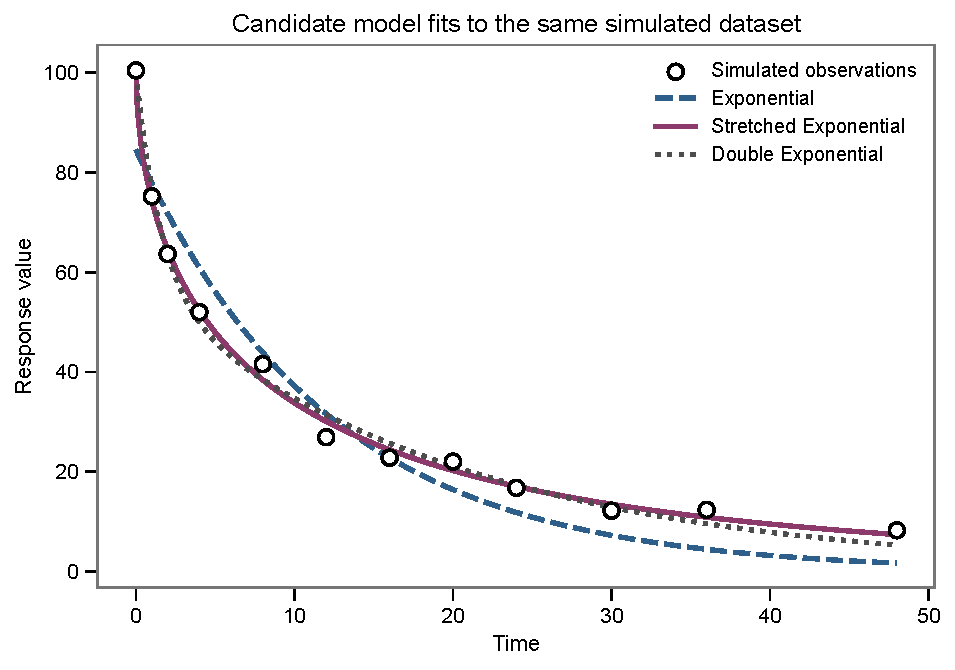
\includegraphics[width=0.92\textwidth]{tutorial/generated/fitted_curves.pdf}
    \caption{Candidate models fitted to the same simulated dataset.}
    \label{fig:tutorial-fitted-curves}
\end{figure}

\subsection{Compare fit metrics, model complexity, and cross-validation}

Table~\ref{tab:tutorial-model-summary} reports goodness-of-fit metrics, AIC\textsubscript{c} comparisons, shuffle-split cross-validation error, and a compact parameter-correlation summary. These quantities answer different questions. \(R^2\), RMSE, and MAE describe agreement with the fitted observations. AIC\textsubscript{c} compares relative empirical support while penalizing additional fitted parameters. Cross-validation RMSE describes prediction error for observations omitted under the selected shuffle-split pattern. The ratio of cross-validation RMSE to full-fit RMSE provides a simple indication of how much prediction error increases when part of the dataset is excluded from fitting.

\begin{table}[htbp]
\centering
\caption{Model-comparison summary generated by the tutorial script. Lower values are preferable for RMSE, MAE, AIC\textsubscript{c}, Delta AIC\textsubscript{c}, and CV RMSE; higher values are preferable for \(R^2\) and AIC\textsubscript{c} weight.}
\label{tab:tutorial-model-summary}
\scriptsize
\setlength{\tabcolsep}{3.5pt}
\begin{tabular}{@{}lrrrrrrrr@{}}
\toprule
\textbf{Model} & \(R^2\) & \textbf{Adj.} \(R^2\) & \textbf{RMSE} & \textbf{MAE} & \textbf{AIC\textsubscript{c}} & \textbf{Delta} & \textbf{CV RMSE} & \textbf{CV/fit} \\
\midrule
\csvreader[head to column names, late after line=\\]{tutorial/generated/model_summary.csv}{}{%
\model & \rtwo & \adjrtwo & \rmse & \mae & \aicc & \deltaaicc & \cvrmse & \cvrmseratio
}
\bottomrule
\end{tabular}
\end{table}

\textit{Suggested discussion to edit:} The exponential fit can still have a high \(R^2\) because it captures most of the large response change, even when its residuals show a systematic pattern. The stretched-exponential fit provides the strongest balance of fit, AIC\textsubscript{c} support, and cross-validation behavior in the default realization. The double-exponential fit is visually competitive, but its additional parameter does not provide enough improvement to offset the complexity penalty, and its cross-validation error increases more relative to its full-fit error.

Figure~\ref{fig:tutorial-cv-predictions} shows the mean prediction for each observation when that observation was placed in the test subset across repeated shuffle splits. Error bars show the variation among held-out predictions. Shuffle split is a general sensitivity check of prediction performance under repeated random omissions; it is not a time-aware forecasting test.

\begin{figure}[htbp]
    \centering
    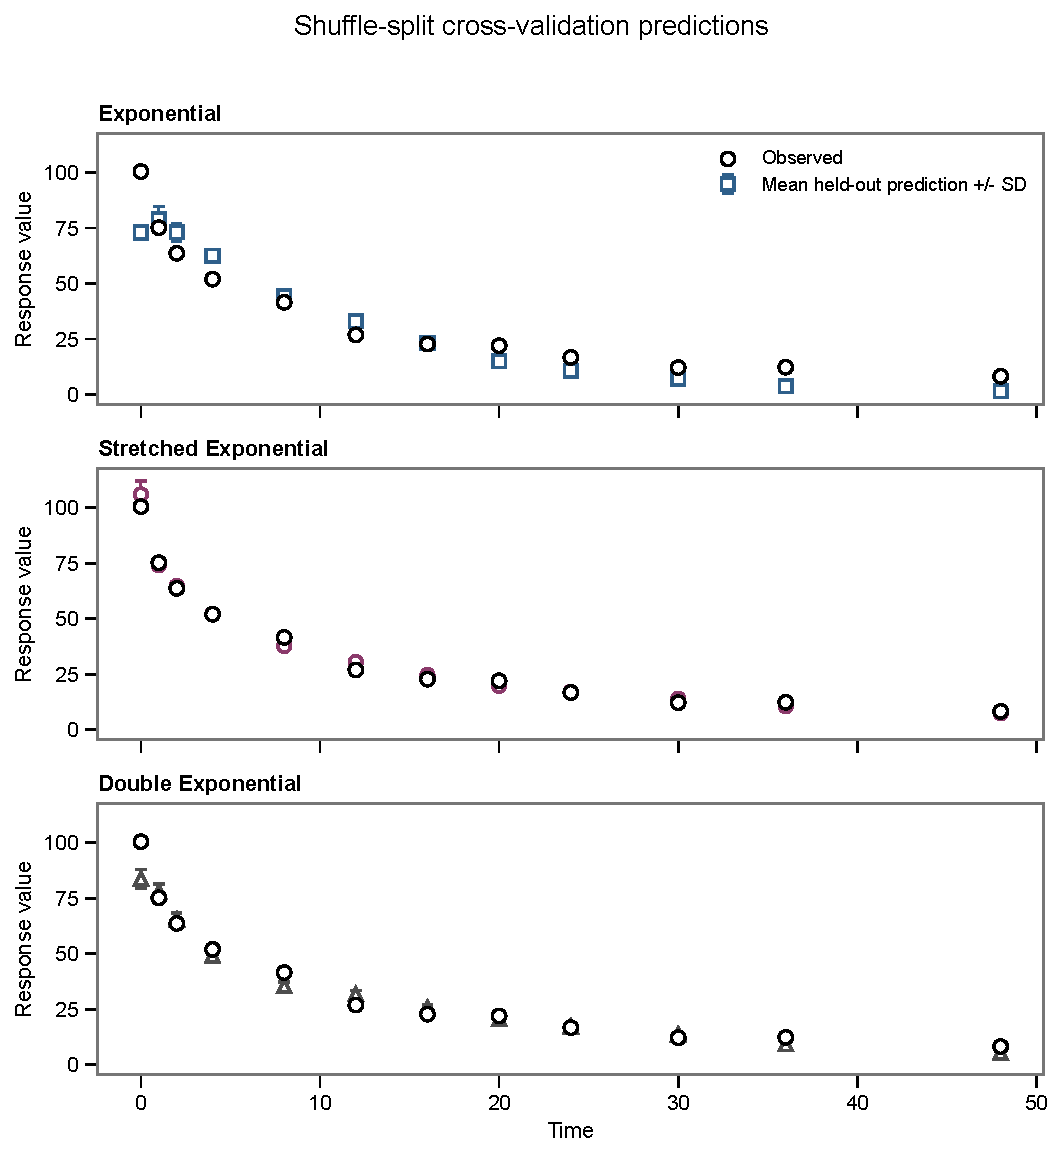
\includegraphics[width=0.92\textwidth]{tutorial/generated/cross_validation_predictions.pdf}
    \caption{Observed responses and held-out predictions from shuffle-split cross-validation. Error bars show the standard deviation of the predictions obtained for each observation across splits in which it was omitted from fitting.}
    \label{fig:tutorial-cv-predictions}
\end{figure}

\subsection{Use residuals versus time to look for missed structure}

Residuals are calculated as observed minus predicted response. A suitable fitted form generally leaves residuals distributed around zero without sustained curvature or adjacent groups that remain mainly above or below zero. Figure~\ref{fig:tutorial-residuals} uses the same y-axis range for all three models so the sizes and patterns can be compared directly.

\begin{figure}[htbp]
    \centering
    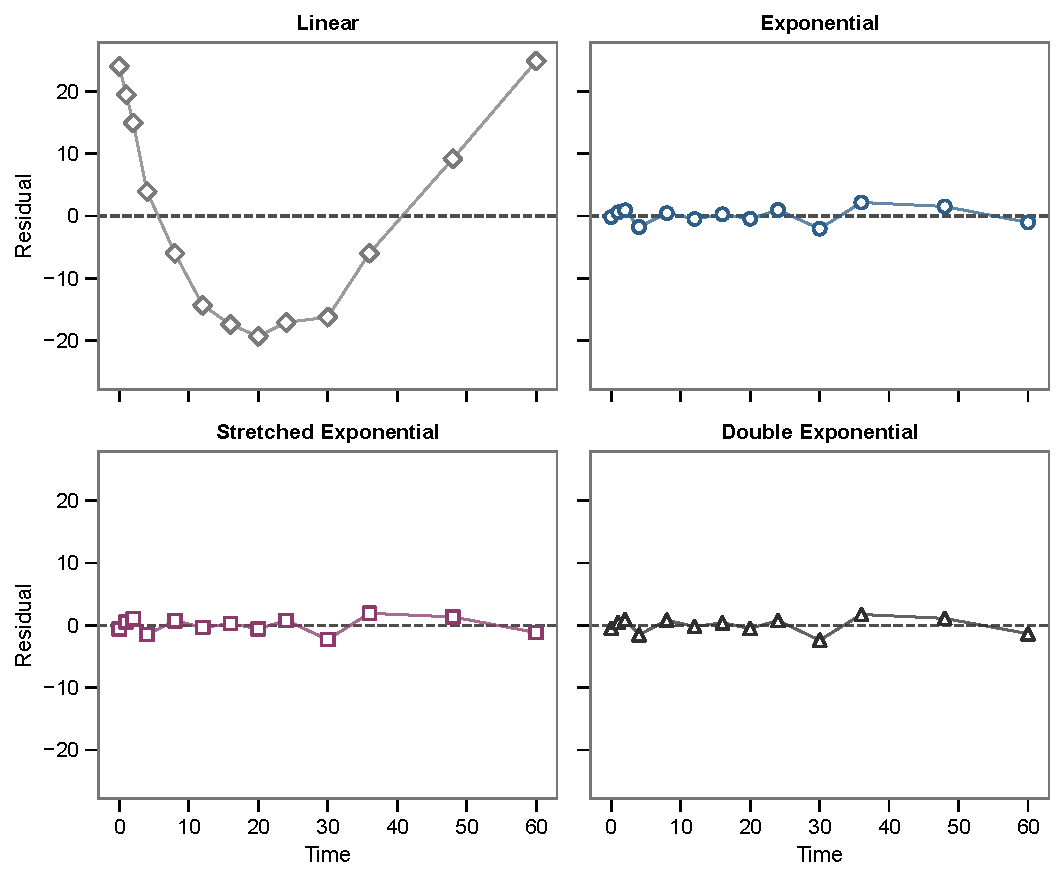
\includegraphics[width=0.92\textwidth]{tutorial/generated/residuals_vs_time.pdf}
    \caption{Residuals versus time for the three fitted models.}
    \label{fig:tutorial-residuals}
\end{figure}

\textit{Suggested discussion to edit:} The exponential residuals show a systematic pattern across time, indicating that the model captures the broad trend but not the detailed curve shape. The stretched-exponential residuals are smaller and do not show the same sustained structure. The double-exponential residuals are also small, but residual size alone does not establish that its additional parameters are well supported.

\subsection{Use Q--Q plots to review residual distribution shape}

A normal Q--Q plot compares ordered standardized residuals with the quantiles expected from a normal distribution. Points close to the reference line are broadly consistent with the assumed residual distribution. Curvature, separation at the ends, or an isolated point can draw attention to skewness, heavy tails, or an unusual residual. With a small dataset, the plot has limited resolution and is interpreted together with the residual-versus-time plot rather than as a formal confirmation of normality.

\begin{figure}[htbp]
    \centering
    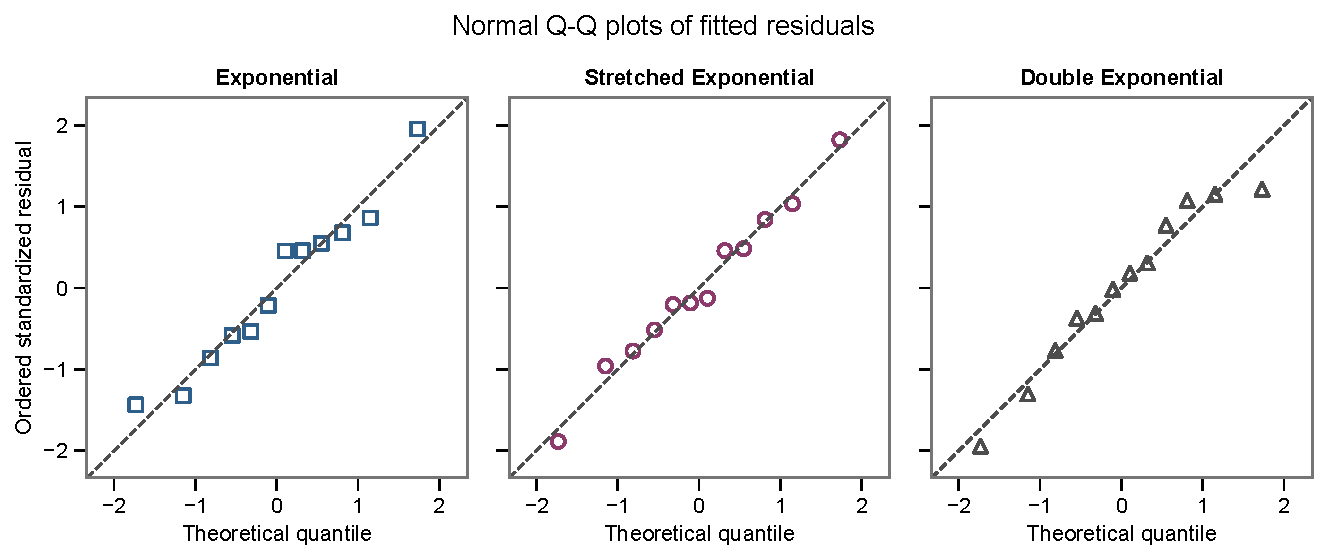
\includegraphics[width=0.98\textwidth]{tutorial/generated/qq_plots.pdf}
    \caption{Normal Q--Q plots of standardized residuals.}
    \label{fig:tutorial-qq}
\end{figure}

\textit{Suggested discussion to edit:} The Q--Q plots do not necessarily distinguish the candidates as clearly as the residual-versus-time plots. That difference is useful: a Q--Q plot addresses residual distribution shape, whereas the residual-versus-time plot is more directly informative about systematic model-form error across the observed profile.

\subsection{Review fitted-parameter uncertainty}

The app reports each fitted parameter with an approximate 95\% confidence-interval half-width. Table~\ref{tab:tutorial-parameters} also reports the standard error and relative standard error. The largest absolute pairwise parameter correlation for each model is included in the generated model-summary CSV. Strong correlation can indicate that different combinations of parameter values produce similar fitted curves, particularly in more flexible nonlinear models.

\begin{longtable}{@{}llrrrr@{}}
\caption{Fitted-parameter estimates and approximate uncertainty.}\label{tab:tutorial-parameters}\\
\toprule
\textbf{Model} & \textbf{Parameter} & \textbf{Estimate} & \textbf{SE} & \textbf{95\% half-width} & \textbf{RSE (\%)} \\
\midrule
\endfirsthead
\toprule
\textbf{Model} & \textbf{Parameter} & \textbf{Estimate} & \textbf{SE} & \textbf{95\% half-width} & \textbf{RSE (\%)} \\
\midrule
\endhead
\csvreader[head to column names, late after line=\\]{tutorial/generated/parameter_estimates.csv}{}{%
\model & \parameter & \estimate & \standarderror & \cihalfwidth & \relativestandarderror
}
\bottomrule
\end{longtable}

\textit{Suggested discussion to edit:} The stretched-exponential parameters are estimated with comparatively narrow intervals in the default realization. The double-exponential fit shows stronger parameter coupling and wider uncertainty for some component parameters. This illustrates why a close fitted curve does not necessarily support mechanistic interpretation of every fitted parameter.

\subsection{Integrated interpretation}

No single output determines the preferred candidate. In the default realization, the exponential model is simple and follows the broad decay trend, but its residual pattern indicates missed structure. The double-exponential model is flexible enough to fit the data closely, but information criteria, cross-validation behavior, and parameter diagnostics provide reasons to question whether the added complexity is supported. The stretched-exponential model provides the strongest overall balance because it captures the curve shape, leaves less systematic residual structure, performs comparatively well under shuffle-split cross-validation, and estimates its parameters with reasonable precision.

For an experimental analysis, the same workflow can be applied without knowing the generating model: inspect the fitted curves, compare complementary metrics, review cross-validation as a sensitivity diagnostic, examine residual-versus-time and Q--Q plots, and consider parameter uncertainty and scientific plausibility before documenting the user-selected model.

%
% Generate the referenced files with:
%   python docs/tutorial/generate_model_comparison_tutorial.py
%
% This file intentionally reads the generated CSV files directly. There is no
% intermediate generated TeX include.

\section{Worked Example: Comparing Candidate Models}
\label{app:model-comparison-tutorial}

\subsection{Purpose of the example}

This worked example illustrates how fitted curves, performance metrics, cross-validation, residual plots, Q--Q plots, and parameter-uncertainty results can be considered together when comparing candidate models. The dataset is simulated so the underlying relationship is known, but the comparison is presented in the same way as an analysis of an unknown experimental relationship. The example is intended as a practical demonstration, not as an acceptance procedure or a set of model-selection criteria.

The accompanying Python script generates one noisy stretched-exponential decay dataset and fits three candidate models available in the app:

\begin{itemize}
    \item an exponential model, used as a relatively simple candidate that captures the broad decay trend but can miss shape details;
    \item a stretched-exponential model, which matches the form used to generate the data; and
    \item a double-exponential model, used to illustrate how additional flexibility can improve or preserve visual fit while increasing model complexity and parameter coupling.
\end{itemize}

The script uses the model registry, fitting functions, performance metrics, shuffle-split cross-validation constructor, and relative-evidence calculations used by the app. The figures use a simplified publication layout rather than reproducing the interactive app display exactly.

\subsection{Simulated dataset and analysis settings}

The generated relationship has the form

\[
    y = a\exp\left(b t^c\right) + \varepsilon,
\]

where \(\varepsilon\) is independent Gaussian noise. The random seed, parameter values, noise level, and cross-validation settings are fixed by default so the example is reproducible. They can be changed near the top of the Python script or through its command-line options.

\begin{longtable}{@{}>{\raggedright\arraybackslash}p{0.38\textwidth}>{\raggedright\arraybackslash}p{0.52\textwidth}@{}}
\toprule
\textbf{Setting} & \textbf{Value} \\
\midrule
\endfirsthead
\toprule
\textbf{Setting} & \textbf{Value} \\
\midrule
\endhead
\csvreader[head to column names, late after line=\\]{tutorial/generated/tutorial_settings.csv}{}{%
\settingname & \settingvalue
}
\bottomrule
\end{longtable}

The simulated observations are listed below. The true response is included only because this is a simulation; it would not be available for an experimental dataset.

\begin{longtable}{@{}rrr@{}}
\toprule
\textbf{Time} & \textbf{True response} & \textbf{Observed response} \\
\midrule
\endfirsthead
\toprule
\textbf{Time} & \textbf{True response} & \textbf{Observed response} \\
\midrule
\endhead
\csvreader[head to column names, late after line=\\]{tutorial/generated/simulated_data.csv}{}{%
\time & \trueresponse & \observedresponse
}
\bottomrule
\end{longtable}

\subsection{Start with the fitted curves}

Figure~\ref{fig:tutorial-fitted-curves} shows the same observations with all three fitted curves. The fitted-curve display is the first opportunity to identify clearly implausible behavior, but models that differ meaningfully can appear similar when the response scale is large relative to the residual differences. For this example, the exponential model follows the overall decline, while the other two models have enough flexibility to represent the curvature more closely.

\begin{figure}[htbp]
    \centering
    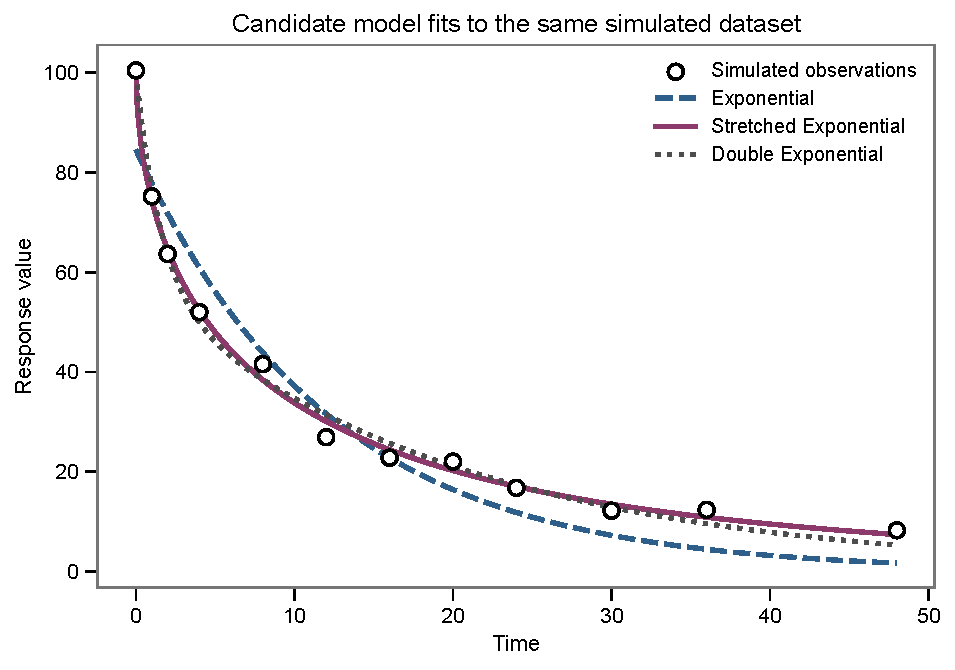
\includegraphics[width=0.92\textwidth]{tutorial/generated/fitted_curves.pdf}
    \caption{Candidate models fitted to the same simulated dataset.}
    \label{fig:tutorial-fitted-curves}
\end{figure}

\subsection{Compare fit metrics, model complexity, and cross-validation}

Table~\ref{tab:tutorial-model-summary} reports goodness-of-fit metrics, AIC\textsubscript{c} comparisons, shuffle-split cross-validation error, and a compact parameter-correlation summary. These quantities answer different questions. \(R^2\), RMSE, and MAE describe agreement with the fitted observations. AIC\textsubscript{c} compares relative empirical support while penalizing additional fitted parameters. Cross-validation RMSE describes prediction error for observations omitted under the selected shuffle-split pattern. The ratio of cross-validation RMSE to full-fit RMSE provides a simple indication of how much prediction error increases when part of the dataset is excluded from fitting.

\begin{table}[htbp]
\centering
\caption{Model-comparison summary generated by the tutorial script. Lower values are preferable for RMSE, MAE, AIC\textsubscript{c}, Delta AIC\textsubscript{c}, and CV RMSE; higher values are preferable for \(R^2\) and AIC\textsubscript{c} weight.}
\label{tab:tutorial-model-summary}
\scriptsize
\setlength{\tabcolsep}{3.5pt}
\begin{tabular}{@{}lrrrrrrrr@{}}
\toprule
\textbf{Model} & \(R^2\) & \textbf{Adj.} \(R^2\) & \textbf{RMSE} & \textbf{MAE} & \textbf{AIC\textsubscript{c}} & \textbf{Delta} & \textbf{CV RMSE} & \textbf{CV/fit} \\
\midrule
\csvreader[head to column names, late after line=\\]{tutorial/generated/model_summary.csv}{}{%
\model & \rtwo & \adjrtwo & \rmse & \mae & \aicc & \deltaaicc & \cvrmse & \cvrmseratio
}
\bottomrule
\end{tabular}
\end{table}

\textit{Suggested discussion to edit:} The exponential fit can still have a high \(R^2\) because it captures most of the large response change, even when its residuals show a systematic pattern. The stretched-exponential fit provides the strongest balance of fit, AIC\textsubscript{c} support, and cross-validation behavior in the default realization. The double-exponential fit is visually competitive, but its additional parameter does not provide enough improvement to offset the complexity penalty, and its cross-validation error increases more relative to its full-fit error.

Figure~\ref{fig:tutorial-cv-predictions} shows the mean prediction for each observation when that observation was placed in the test subset across repeated shuffle splits. Error bars show the variation among held-out predictions. Shuffle split is a general sensitivity check of prediction performance under repeated random omissions; it is not a time-aware forecasting test.

\begin{figure}[htbp]
    \centering
    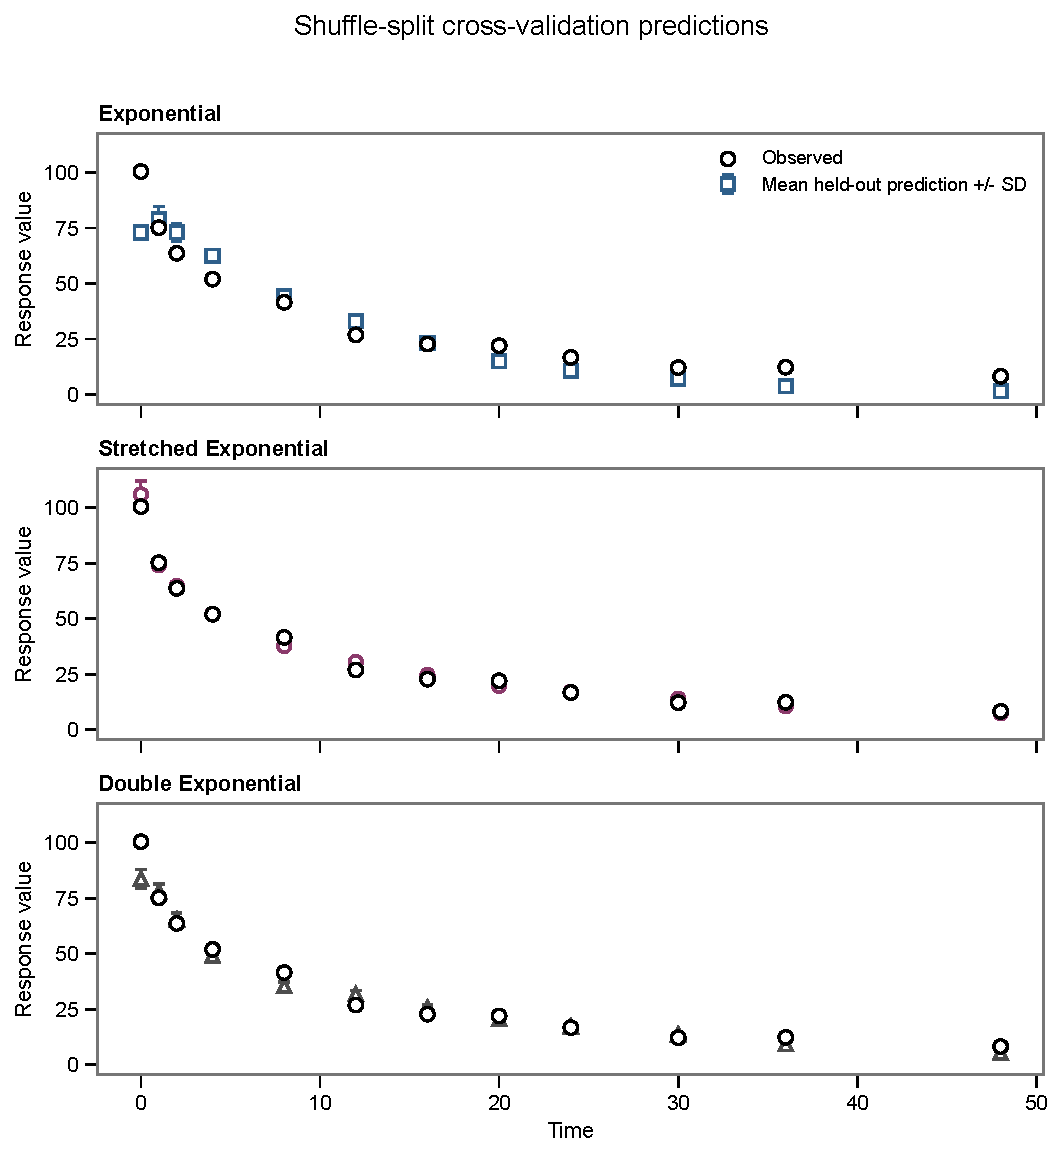
\includegraphics[width=0.92\textwidth]{tutorial/generated/cross_validation_predictions.pdf}
    \caption{Observed responses and held-out predictions from shuffle-split cross-validation. Error bars show the standard deviation of the predictions obtained for each observation across splits in which it was omitted from fitting.}
    \label{fig:tutorial-cv-predictions}
\end{figure}

\subsection{Use residuals versus time to look for missed structure}

Residuals are calculated as observed minus predicted response. A suitable fitted form generally leaves residuals distributed around zero without sustained curvature or adjacent groups that remain mainly above or below zero. Figure~\ref{fig:tutorial-residuals} uses the same y-axis range for all three models so the sizes and patterns can be compared directly.

\begin{figure}[htbp]
    \centering
    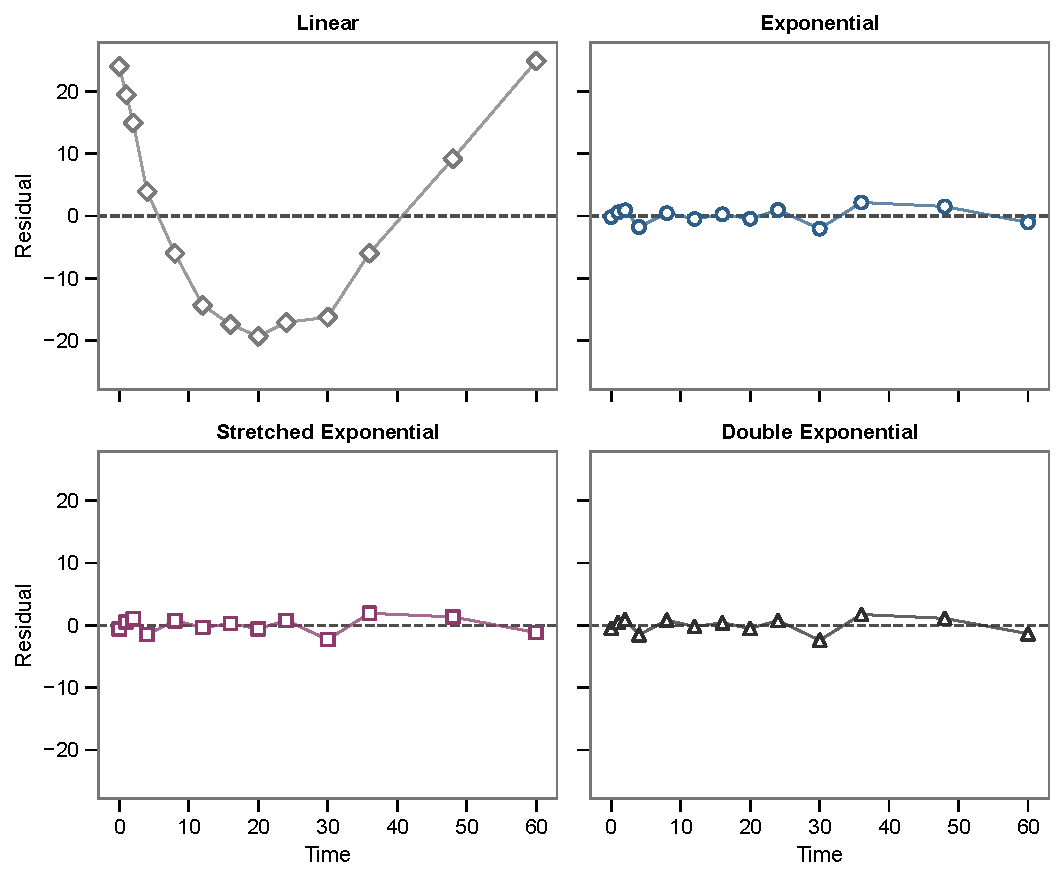
\includegraphics[width=0.92\textwidth]{tutorial/generated/residuals_vs_time.pdf}
    \caption{Residuals versus time for the three fitted models.}
    \label{fig:tutorial-residuals}
\end{figure}

\textit{Suggested discussion to edit:} The exponential residuals show a systematic pattern across time, indicating that the model captures the broad trend but not the detailed curve shape. The stretched-exponential residuals are smaller and do not show the same sustained structure. The double-exponential residuals are also small, but residual size alone does not establish that its additional parameters are well supported.

\subsection{Use Q--Q plots to review residual distribution shape}

A normal Q--Q plot compares ordered standardized residuals with the quantiles expected from a normal distribution. Points close to the reference line are broadly consistent with the assumed residual distribution. Curvature, separation at the ends, or an isolated point can draw attention to skewness, heavy tails, or an unusual residual. With a small dataset, the plot has limited resolution and is interpreted together with the residual-versus-time plot rather than as a formal confirmation of normality.

\begin{figure}[htbp]
    \centering
    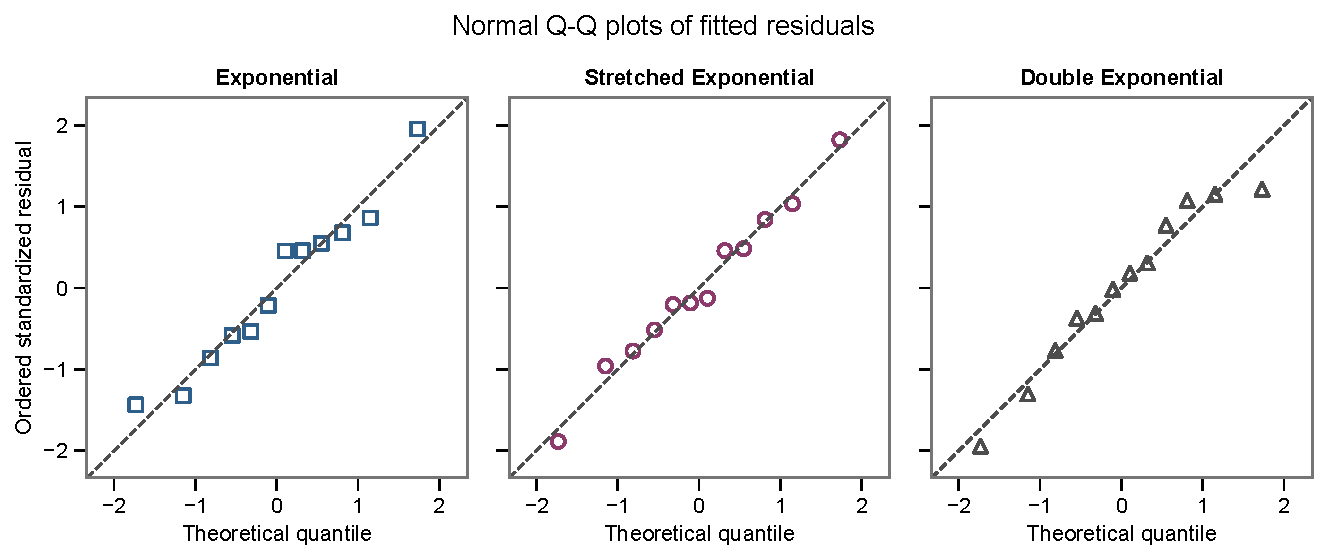
\includegraphics[width=0.98\textwidth]{tutorial/generated/qq_plots.pdf}
    \caption{Normal Q--Q plots of standardized residuals.}
    \label{fig:tutorial-qq}
\end{figure}

\textit{Suggested discussion to edit:} The Q--Q plots do not necessarily distinguish the candidates as clearly as the residual-versus-time plots. That difference is useful: a Q--Q plot addresses residual distribution shape, whereas the residual-versus-time plot is more directly informative about systematic model-form error across the observed profile.

\subsection{Review fitted-parameter uncertainty}

The app reports each fitted parameter with an approximate 95\% confidence-interval half-width. Table~\ref{tab:tutorial-parameters} also reports the standard error and relative standard error. The largest absolute pairwise parameter correlation for each model is included in the generated model-summary CSV. Strong correlation can indicate that different combinations of parameter values produce similar fitted curves, particularly in more flexible nonlinear models.

\begin{longtable}{@{}llrrrr@{}}
\caption{Fitted-parameter estimates and approximate uncertainty.}\label{tab:tutorial-parameters}\\
\toprule
\textbf{Model} & \textbf{Parameter} & \textbf{Estimate} & \textbf{SE} & \textbf{95\% half-width} & \textbf{RSE (\%)} \\
\midrule
\endfirsthead
\toprule
\textbf{Model} & \textbf{Parameter} & \textbf{Estimate} & \textbf{SE} & \textbf{95\% half-width} & \textbf{RSE (\%)} \\
\midrule
\endhead
\csvreader[head to column names, late after line=\\]{tutorial/generated/parameter_estimates.csv}{}{%
\model & \parameter & \estimate & \standarderror & \cihalfwidth & \relativestandarderror
}
\bottomrule
\end{longtable}

\textit{Suggested discussion to edit:} The stretched-exponential parameters are estimated with comparatively narrow intervals in the default realization. The double-exponential fit shows stronger parameter coupling and wider uncertainty for some component parameters. This illustrates why a close fitted curve does not necessarily support mechanistic interpretation of every fitted parameter.

\subsection{Integrated interpretation}

No single output determines the preferred candidate. In the default realization, the exponential model is simple and follows the broad decay trend, but its residual pattern indicates missed structure. The double-exponential model is flexible enough to fit the data closely, but information criteria, cross-validation behavior, and parameter diagnostics provide reasons to question whether the added complexity is supported. The stretched-exponential model provides the strongest overall balance because it captures the curve shape, leaves less systematic residual structure, performs comparatively well under shuffle-split cross-validation, and estimates its parameters with reasonable precision.

For an experimental analysis, the same workflow can be applied without knowing the generating model: inspect the fitted curves, compare complementary metrics, review cross-validation as a sensitivity diagnostic, examine residual-versus-time and Q--Q plots, and consider parameter uncertainty and scientific plausibility before documenting the user-selected model.

%
% Generate the referenced files with:
%   python docs/tutorial/generate_model_comparison_tutorial.py
%
% This file intentionally reads the generated CSV files directly. There is no
% intermediate generated TeX include.

\section{Worked Example: Comparing Candidate Models}
\label{app:model-comparison-tutorial}

\subsection{Purpose of the example}

This worked example illustrates how fitted curves, performance metrics, cross-validation, residual plots, Q--Q plots, and parameter-uncertainty results can be considered together when comparing candidate models. The dataset is simulated so the underlying relationship is known, but the comparison is presented in the same way as an analysis of an unknown experimental relationship. The example is intended as a practical demonstration, not as an acceptance procedure or a set of model-selection criteria.

The accompanying Python script generates one noisy stretched-exponential decay dataset and fits three candidate models available in the app:

\begin{itemize}
    \item an exponential model, used as a relatively simple candidate that captures the broad decay trend but can miss shape details;
    \item a stretched-exponential model, which matches the form used to generate the data; and
    \item a double-exponential model, used to illustrate how additional flexibility can improve or preserve visual fit while increasing model complexity and parameter coupling.
\end{itemize}

The script uses the model registry, fitting functions, performance metrics, shuffle-split cross-validation constructor, and relative-evidence calculations used by the app. The figures use a simplified publication layout rather than reproducing the interactive app display exactly.

\subsection{Simulated dataset and analysis settings}

The generated relationship has the form

\[
    y = a\exp\left(b t^c\right) + \varepsilon,
\]

where \(\varepsilon\) is independent Gaussian noise. The random seed, parameter values, noise level, and cross-validation settings are fixed by default so the example is reproducible. They can be changed near the top of the Python script or through its command-line options.

\begin{longtable}{@{}>{\raggedright\arraybackslash}p{0.38\textwidth}>{\raggedright\arraybackslash}p{0.52\textwidth}@{}}
\toprule
\textbf{Setting} & \textbf{Value} \\
\midrule
\endfirsthead
\toprule
\textbf{Setting} & \textbf{Value} \\
\midrule
\endhead
\csvreader[head to column names, late after line=\\]{tutorial/generated/tutorial_settings.csv}{}{%
\settingname & \settingvalue
}
\bottomrule
\end{longtable}

The simulated observations are listed below. The true response is included only because this is a simulation; it would not be available for an experimental dataset.

\begin{longtable}{@{}rrr@{}}
\toprule
\textbf{Time} & \textbf{True response} & \textbf{Observed response} \\
\midrule
\endfirsthead
\toprule
\textbf{Time} & \textbf{True response} & \textbf{Observed response} \\
\midrule
\endhead
\csvreader[head to column names, late after line=\\]{tutorial/generated/simulated_data.csv}{}{%
\time & \trueresponse & \observedresponse
}
\bottomrule
\end{longtable}

\subsection{Start with the fitted curves}

Figure~\ref{fig:tutorial-fitted-curves} shows the same observations with all three fitted curves. The fitted-curve display is the first opportunity to identify clearly implausible behavior, but models that differ meaningfully can appear similar when the response scale is large relative to the residual differences. For this example, the exponential model follows the overall decline, while the other two models have enough flexibility to represent the curvature more closely.

\begin{figure}[htbp]
    \centering
    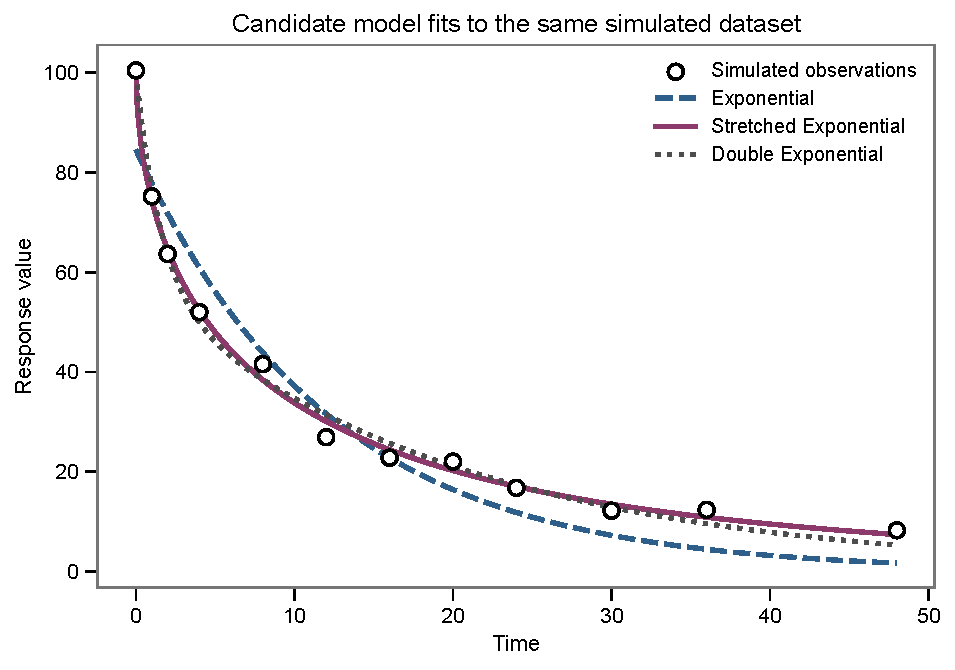
\includegraphics[width=0.92\textwidth]{tutorial/generated/fitted_curves.pdf}
    \caption{Candidate models fitted to the same simulated dataset.}
    \label{fig:tutorial-fitted-curves}
\end{figure}

\subsection{Compare fit metrics, model complexity, and cross-validation}

Table~\ref{tab:tutorial-model-summary} reports goodness-of-fit metrics, AIC\textsubscript{c} comparisons, shuffle-split cross-validation error, and a compact parameter-correlation summary. These quantities answer different questions. \(R^2\), RMSE, and MAE describe agreement with the fitted observations. AIC\textsubscript{c} compares relative empirical support while penalizing additional fitted parameters. Cross-validation RMSE describes prediction error for observations omitted under the selected shuffle-split pattern. The ratio of cross-validation RMSE to full-fit RMSE provides a simple indication of how much prediction error increases when part of the dataset is excluded from fitting.

\begin{table}[htbp]
\centering
\caption{Model-comparison summary generated by the tutorial script. Lower values are preferable for RMSE, MAE, AIC\textsubscript{c}, Delta AIC\textsubscript{c}, and CV RMSE; higher values are preferable for \(R^2\) and AIC\textsubscript{c} weight.}
\label{tab:tutorial-model-summary}
\scriptsize
\setlength{\tabcolsep}{3.5pt}
\begin{tabular}{@{}lrrrrrrrr@{}}
\toprule
\textbf{Model} & \(R^2\) & \textbf{Adj.} \(R^2\) & \textbf{RMSE} & \textbf{MAE} & \textbf{AIC\textsubscript{c}} & \textbf{Delta} & \textbf{CV RMSE} & \textbf{CV/fit} \\
\midrule
\csvreader[head to column names, late after line=\\]{tutorial/generated/model_summary.csv}{}{%
\model & \rtwo & \adjrtwo & \rmse & \mae & \aicc & \deltaaicc & \cvrmse & \cvrmseratio
}
\bottomrule
\end{tabular}
\end{table}

\textit{Suggested discussion to edit:} The exponential fit can still have a high \(R^2\) because it captures most of the large response change, even when its residuals show a systematic pattern. The stretched-exponential fit provides the strongest balance of fit, AIC\textsubscript{c} support, and cross-validation behavior in the default realization. The double-exponential fit is visually competitive, but its additional parameter does not provide enough improvement to offset the complexity penalty, and its cross-validation error increases more relative to its full-fit error.

Figure~\ref{fig:tutorial-cv-predictions} shows the mean prediction for each observation when that observation was placed in the test subset across repeated shuffle splits. Error bars show the variation among held-out predictions. Shuffle split is a general sensitivity check of prediction performance under repeated random omissions; it is not a time-aware forecasting test.

\begin{figure}[htbp]
    \centering
    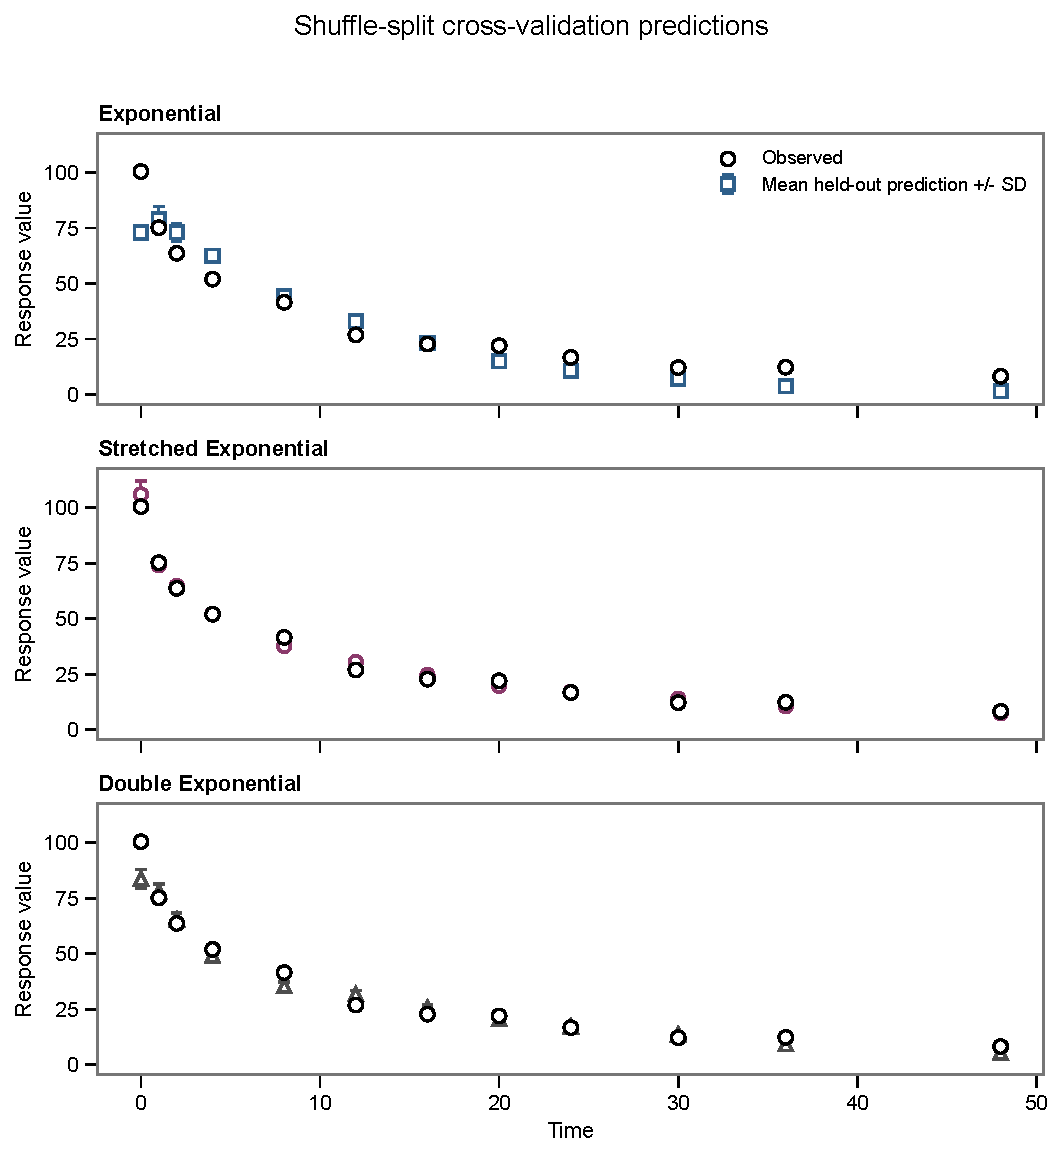
\includegraphics[width=0.92\textwidth]{tutorial/generated/cross_validation_predictions.pdf}
    \caption{Observed responses and held-out predictions from shuffle-split cross-validation. Error bars show the standard deviation of the predictions obtained for each observation across splits in which it was omitted from fitting.}
    \label{fig:tutorial-cv-predictions}
\end{figure}

\subsection{Use residuals versus time to look for missed structure}

Residuals are calculated as observed minus predicted response. A suitable fitted form generally leaves residuals distributed around zero without sustained curvature or adjacent groups that remain mainly above or below zero. Figure~\ref{fig:tutorial-residuals} uses the same y-axis range for all three models so the sizes and patterns can be compared directly.

\begin{figure}[htbp]
    \centering
    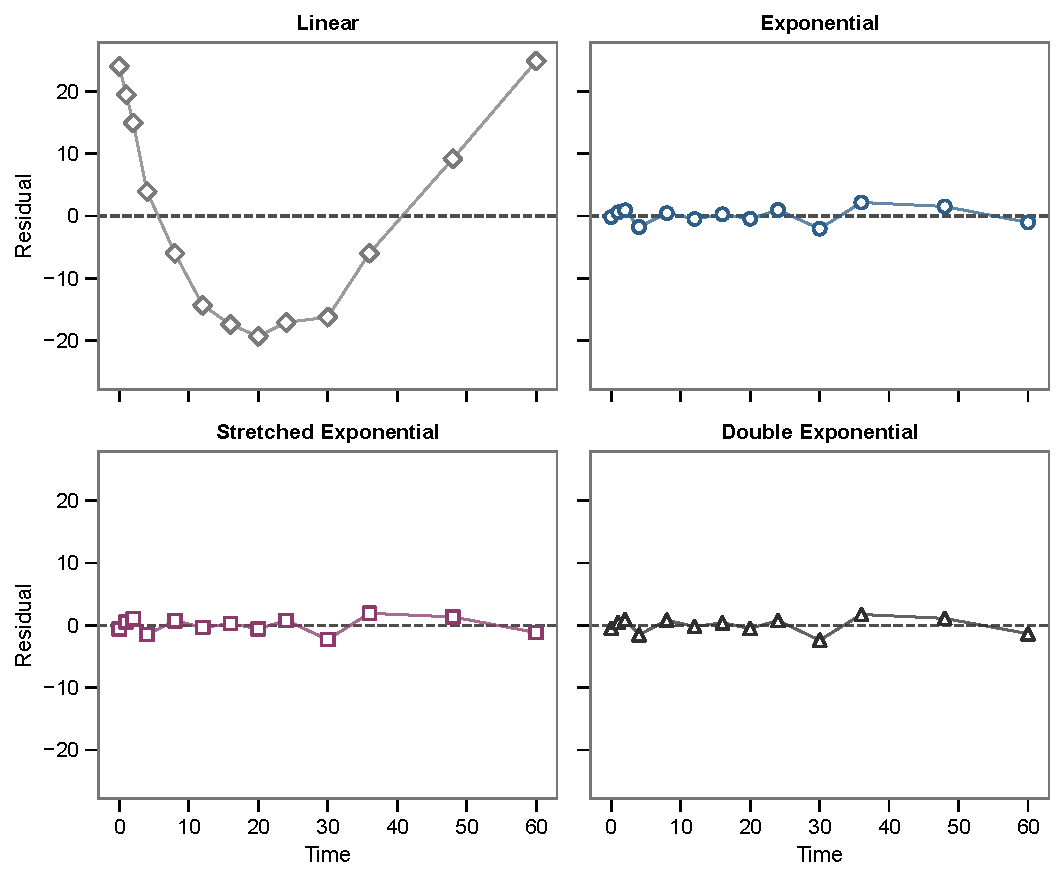
\includegraphics[width=0.92\textwidth]{tutorial/generated/residuals_vs_time.pdf}
    \caption{Residuals versus time for the three fitted models.}
    \label{fig:tutorial-residuals}
\end{figure}

\textit{Suggested discussion to edit:} The exponential residuals show a systematic pattern across time, indicating that the model captures the broad trend but not the detailed curve shape. The stretched-exponential residuals are smaller and do not show the same sustained structure. The double-exponential residuals are also small, but residual size alone does not establish that its additional parameters are well supported.

\subsection{Use Q--Q plots to review residual distribution shape}

A normal Q--Q plot compares ordered standardized residuals with the quantiles expected from a normal distribution. Points close to the reference line are broadly consistent with the assumed residual distribution. Curvature, separation at the ends, or an isolated point can draw attention to skewness, heavy tails, or an unusual residual. With a small dataset, the plot has limited resolution and is interpreted together with the residual-versus-time plot rather than as a formal confirmation of normality.

\begin{figure}[htbp]
    \centering
    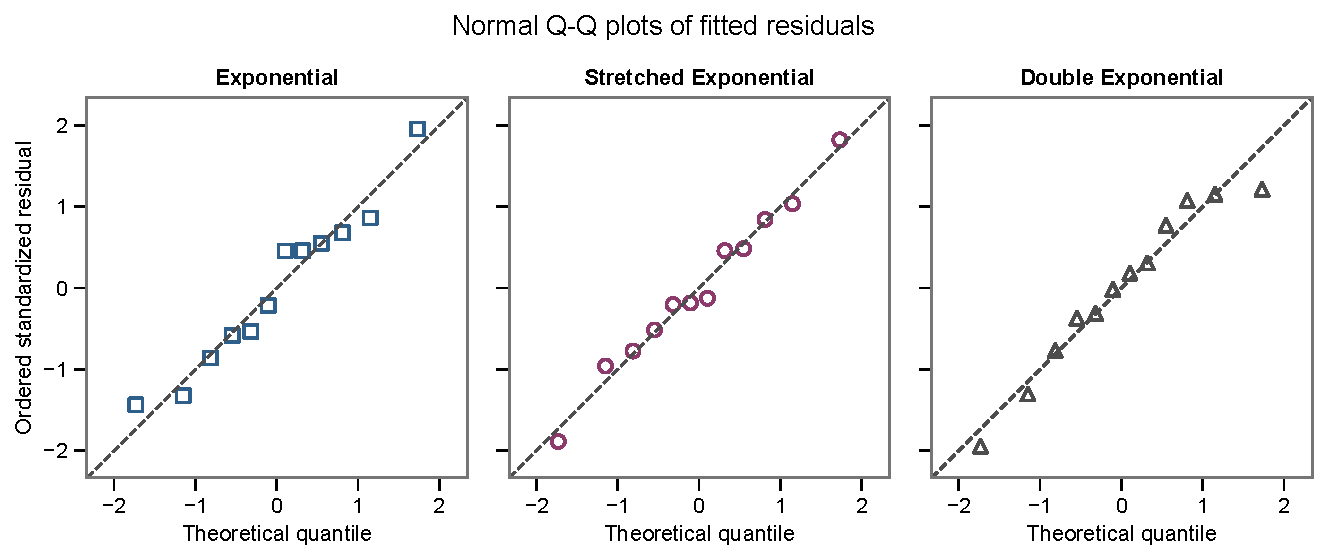
\includegraphics[width=0.98\textwidth]{tutorial/generated/qq_plots.pdf}
    \caption{Normal Q--Q plots of standardized residuals.}
    \label{fig:tutorial-qq}
\end{figure}

\textit{Suggested discussion to edit:} The Q--Q plots do not necessarily distinguish the candidates as clearly as the residual-versus-time plots. That difference is useful: a Q--Q plot addresses residual distribution shape, whereas the residual-versus-time plot is more directly informative about systematic model-form error across the observed profile.

\subsection{Review fitted-parameter uncertainty}

The app reports each fitted parameter with an approximate 95\% confidence-interval half-width. Table~\ref{tab:tutorial-parameters} also reports the standard error and relative standard error. The largest absolute pairwise parameter correlation for each model is included in the generated model-summary CSV. Strong correlation can indicate that different combinations of parameter values produce similar fitted curves, particularly in more flexible nonlinear models.

\begin{longtable}{@{}llrrrr@{}}
\caption{Fitted-parameter estimates and approximate uncertainty.}\label{tab:tutorial-parameters}\\
\toprule
\textbf{Model} & \textbf{Parameter} & \textbf{Estimate} & \textbf{SE} & \textbf{95\% half-width} & \textbf{RSE (\%)} \\
\midrule
\endfirsthead
\toprule
\textbf{Model} & \textbf{Parameter} & \textbf{Estimate} & \textbf{SE} & \textbf{95\% half-width} & \textbf{RSE (\%)} \\
\midrule
\endhead
\csvreader[head to column names, late after line=\\]{tutorial/generated/parameter_estimates.csv}{}{%
\model & \parameter & \estimate & \standarderror & \cihalfwidth & \relativestandarderror
}
\bottomrule
\end{longtable}

\textit{Suggested discussion to edit:} The stretched-exponential parameters are estimated with comparatively narrow intervals in the default realization. The double-exponential fit shows stronger parameter coupling and wider uncertainty for some component parameters. This illustrates why a close fitted curve does not necessarily support mechanistic interpretation of every fitted parameter.

\subsection{Integrated interpretation}

No single output determines the preferred candidate. In the default realization, the exponential model is simple and follows the broad decay trend, but its residual pattern indicates missed structure. The double-exponential model is flexible enough to fit the data closely, but information criteria, cross-validation behavior, and parameter diagnostics provide reasons to question whether the added complexity is supported. The stretched-exponential model provides the strongest overall balance because it captures the curve shape, leaves less systematic residual structure, performs comparatively well under shuffle-split cross-validation, and estimates its parameters with reasonable precision.

For an experimental analysis, the same workflow can be applied without knowing the generating model: inspect the fitted curves, compare complementary metrics, review cross-validation as a sensitivity diagnostic, examine residual-versus-time and Q--Q plots, and consider parameter uncertainty and scientific plausibility before documenting the user-selected model.

\newpage

\section{Glossary}
\label{app:glossary}

This glossary defines terms as they are used in the IVIVC app and this user guide. The definitions are intended as quick references rather than general statistical or regulatory definitions. See Appendix~\ref{app:model-performance} for more detailed interpretation guidance.

\begin{longtable}{@{}>{\raggedright\arraybackslash}p{0.25\textwidth}>{\raggedright\arraybackslash}p{0.67\textwidth}@{}}
\toprule
\textbf{Term} & \textbf{Meaning in this app and guide} \\
\midrule
\endfirsthead
\toprule
\textbf{Term} & \textbf{Meaning in this app and guide} \\
\midrule
\endhead

%Adjusted \(R^2\) & \(R^2\) adjusted for the number of fitted parameters and observations. It can decrease when added parameters do not improve the fit enough to offset the added complexity. \\

%AIC (Akaike information criterion) & Information criterion that balances fit quality against model complexity. Lower values indicate stronger relative support only among comparable models fitted to the same data under the same analysis conditions. \\

%AIC\textsubscript{c} (corrected AIC) & AIC with an additional correction for small samples. It is especially useful when the number of observations is not large relative to the number of fitted parameters. \\

Analysis approach & The overarching method used to establish or evaluate the in vitro/in vivo relationship. An approach can use fitted mathematical models or, for Approach 3, direct interpolation-based mappings. \\

Approach 1: Direct Correlation & Relates in vitro and in vivo times at common response values and fits a model that maps in vitro time to predicted in vivo time. Interpolation by response value can be used when exact response-value matches are unavailable. \\

Approach 2: Independent Model Fitting & Fits the same model family separately to the preprocessed observed in vitro and in vivo datasets, then compares or applies the fitted relationships. Interpolated points are not used for fitting. \\

Approach 3: Direct Mapping & Uses response-at-shared-time and time-at-shared-response-value mappings between the in vitro and in vivo datasets rather than fitting a parametric model. \\

%BIC (Bayesian information criterion) & Information criterion that balances fit quality against model complexity and generally penalizes additional parameters more strongly than AIC as the number of observations increases. Lower values indicate stronger relative support among comparable models. \\

Candidate model & A mathematical form considered for fitting within an applicable analysis approach. Candidate models can differ in shape, number of parameters, and flexibility. \\

Confidence interval (parameter) & Approximate range used to summarize uncertainty in a fitted parameter. The app reports each parameter as the estimate \(\pm\) the half-width of a 95\% confidence interval when the required covariance information is available. \\

%Confidence interval half-width & Distance from a parameter estimate to either endpoint of the reported symmetric confidence interval. This is the value shown after the \(\pm\) sign in the app. \\

Covariance matrix & Matrix calculated from the fitted model that summarizes approximate parameter variances and how parameter estimates vary together. It is used for parameter standard errors, confidence intervals, and parameter-correlation diagnostics. \\

Cross-validation (CV) & Prediction-error and sensitivity diagnostic in which part of the fitting data is set aside, the model is fit to the remaining observations, and predictions are compared with the omitted observations. CV does not estimate parameter uncertainty. \\

%CV comparison badge & Informational label that summarizes whether CV performance is similar to or worse than full-fit performance for eligible metrics. It is a screening aid, not an acceptance criterion. \\

%Delta (information criterion) & Difference between a model's AIC, AIC\textsubscript{c}, or BIC value and the lowest value for the comparable candidate set. A delta near zero indicates support similar to the leading model under that criterion. \\

Densified interpolation & Interpolation option that adds intermediate grid points in both the time and response-value directions before interpolation. The added values are estimates, not additional experimental observations. \\

Empirical support & Relative support provided by the observed data for one candidate model compared with others under a selected information criterion. It does not establish that a model is correct or suitable for a particular use. \\

%Evidence ratio & Ratio comparing the largest information-criterion weight in a candidate set with a model's weight. Larger values indicate less relative support than the leading model. \\

Extrapolation & Use of a fitted model to estimate behavior outside the range of the observed data. Extrapolated behavior generally has greater uncertainty and depends more strongly on the assumed model form. \\

Fit/CV ratio & Ratio of a full-fit metric value to the corresponding mean cross-validation metric reported by the app. Values near 1 indicate similar full-fit and cross-validation performance; interpretation also depends on the metric and CV scheme. \\

Fitted model & A candidate model after its parameters have been estimated from the data. \\

Fitted parameter diagnostics & App summaries that flag large relative standard errors, strong parameter coupling, or combined identifiability concerns for closer review. They do not determine whether a model is valid or acceptable. \\

Fitting dataset & Required dataset containing paired in vitro and in vivo time-course data used to establish the IVIVC relationship. \\

Full fit & Model fit obtained using the complete fitting dataset rather than a training subset created for cross-validation. \\

Goodness of fit & Degree to which a fitted model describes the observations used to estimate its parameters. The app summarizes goodness of fit with selected metrics and fitted-curve displays. \\

Grid search initialization & Procedure that evaluates many candidate parameter starting values before the final nonlinear least-squares fit and selects a promising starting point. It can improve fitting robustness but does not guarantee a global optimum. \\

Identifiability & Degree to which the available data distinguish among possible values of fitted model parameters. Poor identifiability occurs when substantially different parameter combinations can produce very similar fitted curves. \\

Information criterion & Model-comparison measure, such as AIC, AIC\textsubscript{c}, or BIC, that combines fit quality with a penalty for model complexity. Information-criterion values are interpreted comparatively, not as absolute fit scores. \\

Interpolation & Estimation of response values between measured points. Interpolated values are derived from the observed data and are not new measurements. \\

In vitro & Measurements or behavior observed in a laboratory or other setting outside the living organism. In this app, in vitro data provide one side of the IVIVC relationship. \\

In vivo & Measurements or behavior observed in a living organism. In this app, in vivo data provide the other side of the IVIVC relationship. \\

IVIVC (in vitro--in vivo correlation) & Quantitative relationship between in vitro and in vivo degradation behavior. The app provides several approaches for establishing, evaluating, and applying such relationships. \\

%Leave-contiguous-block-out & Time-aware CV scheme that sets aside a block of adjacent observations in time order and fits the model to the remaining data. It evaluates sensitivity to a missing region of the observed profile. \\

%Leave-one-timepoint-out & CV scheme that sets aside one time point at a time and fits the model using all remaining observations. It preserves as much fitting data as possible for small datasets. \\

%MAE (mean absolute error) & Average absolute difference between observed and fitted or predicted values. Lower values indicate smaller errors, and the units match the response units. \\

Model complexity & Flexibility introduced by a model's form and number of fitted parameters. Additional complexity can improve in-sample fit but can also increase parameter uncertainty or overfitting. \\

Model parameter & Numerical quantity in a model equation that is estimated from the data during fitting, such as an amplitude, rate constant, exponent, or lag parameter. \\

%MSE (mean squared error) & Average squared difference between observed and fitted or predicted values. Lower values indicate smaller errors; the units are squared response units. \\

Normalization & Preprocessing that expresses response values relative to a reference, such as the first response value or the observed minimum and maximum, so datasets can be compared on a common relative scale. \\

Observed-response inverse mapping & Approach 2 prediction method that maps each observed in vitro prediction response to the time at which the fitted in vivo calibration curve reaches that response. The app restricts the inverse to a one-to-one fitted curve over the observed in vivo calibration time range and does not extrapolate response values outside that fitted range. Approximate 95\% inverse-prediction intervals combine fitted in vivo parameter uncertainty with an assumed response uncertainty equal to the in vivo fit's residual standard error. \\

%NRMSE (normalized root mean squared error) & RMSE divided by a selected normalization factor, such as the response mean or standard deviation. Interpretation depends on the normalization method used. \\

Overfitting & Situation in which a model's flexibility allows it to follow random variation in the fitted data rather than only the underlying relationship. Overfitting can appear as excellent full-fit metrics accompanied by poorer CV performance or unstable parameters. \\

Parameter coupling / correlation & Tendency for two fitted parameter estimates to change together. Strong coupling can mean that one parameter can compensate for another while producing a similar fitted curve. \\

Parameter estimate & Fitted numerical value of a model parameter obtained from the optimization procedure. \\

%Parameter identifiability caution & App badge used when strong parameter coupling occurs together with elevated parameter uncertainty or a related numerical sensitivity indication. It signals a need for closer review rather than a pass/fail conclusion. \\

Parameter uncertainty & Uncertainty in the numerical values of fitted model parameters. The app summarizes it with approximate confidence intervals, relative standard errors, and parameter-coupling diagnostics where available. \\

Parametric model & Mathematical model described by an equation with a finite set of fitted parameters. Approaches 1 and 2 can use parametric models; Approach 3 uses direct mappings rather than a fitted parametric model. \\

Prediction band & Model-based interval around a fitted or predicted relationship that incorporates sources of uncertainty defined for the applicable approach. In fitted parametric models, the displayed 95\% prediction band generally includes fitted-parameter uncertainty and residual/model error. \\

Prediction dataset & Optional in vitro dataset used after model fitting to generate corresponding in vivo predictions. \\

Prediction error & Difference between an observed response and the corresponding model prediction. For fitted observations, this difference is also called a residual. \\

Preprocessing & Operations applied to uploaded data before fitting, comparison, or prediction. In this app, preprocessing can include normalization, scaling, and interpolation. \\

Shared-grid interpolation & Interpolation option that estimates response values at the union of observed time points and estimates times at the union of observed response values. Estimates outside the overlapping range are unavailable. \\

Q--Q plot (quantile--quantile plot) & Graph that compares ordered standardized residuals with the quantiles expected from a normal distribution. It is used as a qualitative diagnostic for residual-distribution shape. \\

%\(R^2\) (coefficient of determination) & Measure of how much of the observed response variation is represented by the fitted model relative to a mean-response baseline. Higher values indicate closer agreement with the observed pattern, but a high \(R^2\) does not establish model suitability. \\

Random seed & Starting value used by a pseudorandom procedure so randomized operations, like shuffle split CV and grid search, can be reproduced. \\

Relative model evidence & Comparison of candidate models using AIC, AIC\textsubscript{c}, or BIC, including delta values, weights, and evidence ratios. These quantities describe relative support only within a comparable candidate set. \\

Relative standard error (RSE) & Parameter standard error expressed as a percentage of the absolute parameter estimate. Large RSE values indicate that uncertainty is large relative to the fitted value. \\

Residual & Observed response minus the fitted or predicted response (i.e., the error in a given prediction). Residual patterns over time can reveal systematic lack of fit that is not obvious from the fitted curve alone. \\

Residual plot & Plot of residuals against time or another fitted quantity. In this app, raw residual plots show observed-minus-predicted response values versus time in the original response units. \\

Residual degrees of freedom & Number of fitted observations minus the number of estimated model parameters, \(n-p\). It is used in estimating residual variance and in the app's approximate parameter confidence intervals. \\

Response value & Measured y-axis quantity that changes with time, such as mass remaining, molecular weight, strength, or another degradation-related endpoint. \\

%RMSE (root mean squared error) & Square root of MSE. It summarizes typical error magnitude in the same units as the response and gives greater influence to larger errors than MAE. \\

Scaling & Preprocessing that changes the numerical scale of time or response values, such as applying a base-10 logarithm, without changing which observations are present. \\

Scientific plausibility & Consistency of the fitted relationship, parameter values, and predicted behavior with relevant knowledge of the polymer, degradation mechanism, test conditions, and intended use. \\

%Shuffle split & Default CV scheme that repeatedly divides observations at random into training and test subsets. It provides a general robustness check but does not preserve time order. \\

Standard error (SE) & Approximate standard deviation of a fitted parameter estimate implied by the fitted model and covariance calculation. Smaller values indicate more precise parameter estimates on that parameter's scale. \\

%Support badge & Informational label based on an information-criterion delta value. It summarizes relative model support as a screening aid and is not an acceptance criterion or model recommendation. \\

Test data & Observations set aside during a CV split and used to evaluate predictions from a model fitted without those observations. \\

Time constant (integral time constant) & Characteristic time scale calculated, when finite, as the area under a fitted decay curve after normalizing its fitted value at time zero to 1, $\tau = f(0)^{-1}\int_0^\infty f(t)\,dt$. In Approach 2, in vitro and in vivo time constants can be compared or used as a ratio for time rescaling. \\

Training data & Observations retained during a CV split and used to fit the model for that split. \\

%Weight (information criterion) & Normalized relative-support value calculated from information-criterion deltas across the displayed candidate set. Weights sum to 1 within that set and are not absolute probabilities that a model is correct. \\

\bottomrule
\end{longtable}

\newpage

\addcontentsline{toc}{section}{References}
\bibliographystyle{unsrt}
%\nocite{*}
\bibliography{references}

\end{document}

